%% LyX 2.0.2 created this file.  For more info, see http://www.lyx.org/.
%% Do not edit unless you really know what you are doing.
\documentclass[12pt,letterpaper,english,12pt,english,openany,letterpaper,pagesize]{scrbook}
\usepackage[T1]{fontenc}
\usepackage[latin9]{inputenc}
\setlength{\parskip}{\medskipamount}
\setlength{\parindent}{0pt}
\usepackage{float}
\usepackage{amsthm}
\usepackage{amsmath}
\usepackage{amssymb}
\usepackage{graphicx}
\usepackage{setspace}
\usepackage{esint}
\onehalfspacing

\makeatletter

%%%%%%%%%%%%%%%%%%%%%%%%%%%%%% LyX specific LaTeX commands.
\pdfpageheight\paperheight
\pdfpagewidth\paperwidth

%% Because html converters don't know tabularnewline
\providecommand{\tabularnewline}{\\}

%%%%%%%%%%%%%%%%%%%%%%%%%%%%%% User specified LaTeX commands.
%\documentclass[12pt,spanish,fleqn,openany,letterpaper,pagesize]{scrbook}

%\usepackage[ansinew]{inputenc}
%\usepackage[spanish]{babel}
\usepackage{fancyhdr}
\usepackage{epsfig}
\usepackage{epic}
\usepackage{eepic}
\usepackage{amsmath}
\usepackage{threeparttable}
\usepackage{amscd}
\usepackage{here}
\usepackage{graphicx}
\usepackage{lscape}
\usepackage{tabularx}
\usepackage{subfigure}
\usepackage{longtable}


\usepackage{rotating} %Para rotar texto, objetos y tablas seite. No se ve en DVI solo en PS. Seite 328 Hundebuch
                        %se usa junto con \rotate, \sidewidestable ....


\renewcommand{\theequation}{\thechapter-\arabic{equation}}
\renewcommand{\thefigure}{\textbf{\thechapter-\arabic{figure}}}
\renewcommand{\thetable}{\textbf{\thechapter-\arabic{table}}}


\pagestyle{fancyplain}%\addtolength{\headwidth}{\marginparwidth}
\textheight22.5cm \topmargin0cm \textwidth16.5cm
\oddsidemargin0.5cm \evensidemargin-0.5cm%
\renewcommand{\chaptermark}[1]{\markboth{\thechapter\; #1}{}}
\renewcommand{\sectionmark}[1]{\markright{\thesection\; #1}}
\lhead[\fancyplain{}{\thepage}]{\fancyplain{}{\rightmark}}
\rhead[\fancyplain{}{\leftmark}]{\fancyplain{}{\thepage}}
\fancyfoot{}
\thispagestyle{fancy}%


\addtolength{\headwidth}{0cm}
\unitlength1mm %Define la unidad LE para Figuras
%\mathindent0cm %Define la distancia de las formulas al texto,  fleqn las descentra
\marginparwidth0cm
\parindent0cm %Define la distancia de la primera linea de un parrafo a la margen

%Para tablas,  redefine el backschlash en tablas donde se define la posici\'{o}n del texto en las
%casillas (con \centering \raggedright o \raggedleft)
\newcommand{\PreserveBackslash}[1]{\let\temp=\\#1\let\\=\temp}
\let\PBS=\PreserveBackslash

%Espacio entre lineas
\renewcommand{\baselinestretch}{1.1}

%Neuer Befehl f\"{u}r die Tabelle Eigenschaften der Aktivkohlen
\newcommand{\arr}[1]{\raisebox{1.5ex}[0cm][0cm]{#1}}

%Neue Kommandos
\usepackage{resources/Befehle}


%Trennungsliste
\hyphenation {Reaktor-ab-me-ssun-gen Gas-zu-sa-mmen-set-zung
Raum-gesch-win-dig-keit Durch-fluss Stick-stoff-gemisch
Ad-sorp-tions-tem-pe-ra-tur Klein-schmidt
Kohlen-stoff-Mole-kular-siebe Py-rolysat-aus-beu-te
Trans-port-vor-gan-ge}

%\pagenumbering{roman}
%\let\myTOC\tableofcontents
%\renewcommand\tableofcontents{%
%\myTOC
%\clearpage
%\pagenumbering{arabic}
%}

\makeatother

\usepackage{babel}
\begin{document}
\pagenumbering{roman}
\begin{center}
\begin{figure}
\centering%
%
\includegraphics[width=0.4\columnwidth]{resources/logo_un.png}
%
\includegraphics[width=0.4]{logo_un.png}
\end{figure}
\thispagestyle{empty}

\vspace{2cm}


\textbf{\huge Adapted Laplacian Operator For Hybrid Quad/Triangle
Meshes}{\huge \par}

\vspace{6cm}


\textbf{\large Alexander Pinz�n Fern�ndez}{\large \par}

\vspace{6cm}


Universidad Nacional de Colombia

Facultad de Ingenieria, Departamento de Sistemas e Industrial

{\small Grupo de Investigaci�n CIM@LAB}{\small \par}

Bogot�, Colombia

2014

\end{center}

\newpage{}

\begin{center}
\thispagestyle{empty} 
\vspace*{0cm} 

\textbf{\huge Adapted Laplacian Operator For Hybrid Quad/Triangle
Meshes}{\huge \par}

\vspace{2.5cm}


\textbf{\large Alexander Pinz�n Fern�ndez}{\large \par}

\vspace{2.5cm}


{\small A thesis submitted in partial fulfillment of the requirements
for the degree of:}{\small \par}

\textbf{Master in Systems Engineering and Computer Science}

\vspace{2cm}


{\small Advisor:}\\
{\small Eduardo Romero Castro , Ph.D.}{\small \par}

{\small \vspace{1.5cm}
}{\small \par}

{\small Research Area:}\\
{\small Computer Graphics}{\small \par}

{\small \vspace{2cm}
}{\small \par}

{\small Universidad Nacional de Colombia}\\
{\small Facultad de Ingenieria, Departamento de Sistemas e Industrial}\\
{\small Grupo de Investigaci�n CIM@LAB}\\
{\small Bogot�, Colombia}\\
{\small 2014}{\small \par}

\end{center}
\newpage 
\thispagestyle{empty}

\textbf{Dedicaci�n}

{\small \vspace{4cm}
}{\small \par}

\noindent \begin{flushright}
\begin{minipage}[t]{8cm}%
{\small A Beatriz y Campo Elias mis padres que siempre me dieron la
libertad de escoger, con su comprensi�n y apoyo me permitieron dedicar
mi tiempo a la ciencia.}{\small \par}

{\small \vspace{1cm}
}{\small \par}

{\small A mis padres}{\small \par}

{\small \vspace{1cm}
}{\small \par}

Beatriz Fernandez Vargas

Campo Elias Pinzon Rojas%
\end{minipage}
\par\end{flushright}

\newpage
\thispagestyle{empty}

\textbf{\LARGE Acknowledgement}{\LARGE \par}

\addcontentsline{toc}{chapter}{\numberline{}Acknowledgement}

\vspace{2cm}


I wold like to thank my advisor professor Eduardo Romero and CIM\&LAB
research group for his support in this thesis. 

{\small \vspace{1cm}
}{\small \par}

I would like to thank all the workers in Colombia who fund the public
education with their work.

{\small \vspace{1cm}
}{\small \par}

This work was supported in part by the Blender Foundation, Google
Summer of code program at 2012 - 2013. 

\newpage{}

\textbf{\LARGE Abstract}{\LARGE \par}

\addcontentsline{toc}{chapter}{\numberline{}Abstract}

In the last two decades three-dimensional modeling methods have been
evolving and developing rapidly, thanks in part to the use of vector
operators of differential geometry. The Laplacian operator has been
one of the most widely studied and used thanks to the properties exhibited
by their eigenvectors in novel applications such as noise reduction,
enhancement, remeshing, UV mapping, posed, skeletonization, among
other. The differential operator is defined in a continuous and smooth
domain named manifold, manifolds are often approximated by discrete
polygon meshes composed by triangles and quadrangles which represent
the real world three-dimensional objects. In these meshes spectral
structure is calculated using a discrete Laplacian operator, the discrete
version of the Laplacian operator given by Pinkall in 1993 works only
with meshes of triangles, and Xiong in 2011 working exclusively with
quads. This thesis proposes an original extension of the Laplacian
operator that allows to work with hybrid meshes composed by triangles
and quadrangles.

Along with the operator, this work presents new sculpting and modeling
applications with base on the enhancement, applications on subdivision
surfaces using smoothing, mesh posing using differential coordinates
and skeletonization using iterative contraction. This series of applications
demonstrates the quality, predictability and flexibility of the proposed
operator.

The proposed operator was successfully used in real production environments
within software Blender how new tools. Currently these tools are available
as open source software. 

\textbf{\LARGE Resumen}{\LARGE \par}

En las dos �ltimas d�cadas los m�todos de modelado tridimensional
han ido evolucionando y desarroll�ndose r�pidamente, en parte gracias
al uso de operadores vectoriales de geometr�a diferencial. El operador
Laplaciano ha sido uno de los m�s ampliamente estudiado y usado gracias
a las propiedades exhibidas por sus vectores propios en novedosas
aplicaciones como: reducci�n de ruido, realce, remallado, mapeo UV,
posado, esqueletonizaci�n, entre otras. Este operador diferencial
es definido en un dominio continuo y suave llamado variedad, las variedades
son a menudo aproximadas por mallas discretas de pol�gonos compuestas
por tri�ngulos y cuadr�ngulos que a su vez representan objetos tridimensionales
del mundo real. En estas mallas se calcula la estructura espectral
con el uso de alg�n operador Laplaciano discreto, la versi�n discreta
del operador Laplaciano propuesta por Pinkall en el 1993 trabaja �nicamente
con mallas compuestas por tri�ngulos, y la de Xiong en el 2011 trabaja
exclusivamente con cuadr�ngulos. Esta tesis propone una extensi�n
original del Operador Laplaciano que permite trabajar con mallas h�bridas
compuestas por tri�ngulos y cuadr�ngulos.

Junto con el operador, este trabajo presenta nuevas aplicaciones en
esculpido y modelamiento con base en el realce, aplicaciones en subdivisi�n
de superficies con el uso de suavizado, posado de mallas con el uso
de coordenadas diferenciales y esqueletonizaci�n usando contracci�n
iterativa. Esta serie de aplicaciones demuestra la calidad, predictibilidad
y flexibilidad del operador propuesto.

El operador propuesto fue usado de forma exitosa en ambientes reales
de producci�n dentro del software Blender como nuevas herramientas.
Actualmente estas herramientas est�n disponibles como programas de
c�digo abierto.

{\small \vspace{1cm}
}{\small \par}

\textbf{\small Keywords: laplacian operator; smooth; enhance; sculpting;
subdivision surface}{\small \par}

\tableofcontents{}

\listoffigures


\listoftables


\pagenumbering{arabic}


\chapter{Introduction}

The discrete versions of Laplace Beltrami Operator have been used
in the last years for the develop of new geometric modeling tools.
In the work of Pinkall \cite{Pinkall1993} was introduced the cotangent
version of Laplace operator, that allow to find the minimal surface
when compute a discete harmonic map with the Laplacian operator, this
version has been widely studied and applied in various problems of
computer geometric modeling. The manifolds that are continuous domains
homeomorphic to $\mathbb{R}^{n}$ are represented in computers by
polygon meshes. These polygons are generally composed of triangles
and quadrangles, while work with laplacian operator in this hybrid
composition are not a mathematical challenge, most research uses only
meshes composed by triangles \cite{Pinkall1993,Desbrun1999,Meyer2003,Sorkine2004,Au2008,Belkin2008,Hahne2006},
in other recent studies \cite{Liu2008,Xiong2011} the Laplacian operator
is working exclusively with quadrangles. But in the artistic scope
topology and the way the edges are distributed, the triangle and quadrangles,
directly affects the processes of animation, interpolation, textured,
etc. As discussed by \cite{Mullen2007} who use a manual connection
of a couple of vertices to perform animation processes and interpolation.
It is then of paramount importance to develop operators that easily
interact with such meshes, eliminating the need of preprocessing the
mesh to convert it to triangles and change the original topology. 

Modeling techniques able to generate a variety of realistic shapes,
have been developed \cite{Botsch2006}. Editing techniques have evolved
from affine transformations to advanced tools like sculpting \cite{Coquillart1990,Galyean1991,Stanculescu2011},
editing, creation from sketches \cite{Igarashi1999,Gonen2012}, and
complex interpolation techniques \cite{Sorkine2004,Zhou2005}. Catmull-Clark
based methods however require to interact with a minimun number of
control points for any operation to be efficient, or in other words,
a unicity condition is introduced by demanding a smooth surface after
any of these shape operations. Hence, traditional modeling methods
for subdividing surfaces from coarse geometry have become widely popular
\cite{Catmull1978,Stam1998}. These works have generalized a uniform
B-cubic spline knot insertion to meshes, some of them adding some
type of control, for instance with the use of creases to produce sharp
edges \cite{DeRose1998}, or the modification of some vertex weights
to locally control the zone of influence \cite{Biermann2000}. Neverteless
these methods are difficult to deal with since they require a large
number of parameters and a very tedious customization. Instead, the
presented applications requires a single parameter that controls the
global curvature, which is used to maintain realistic shapes, creating
a family of different versions of the same object and therefore preserving
the detail of the original model and a realistic appearance. 

The shape inflation and shape exaggeration can thus be used as such
brush in the sculpting process, when inflating a shape since current
brushes end up by losing detail when moving vertices \cite{Stanculescu2011}.
In contrast, the presented enhance method inflates a mesh by moving
the vertices towards the reverse curvature direction, conserving the
shape and sharp features of the model.


\paragraph{Contributions}

This work presents an extension of the Laplace Beltrami Operator for
hybrid quad/triangle meshes, representing a larger mesh spectrum from
what has been presented so far. The method eliminates the need of
preprocessing and allows preservation of the original topology. Likewise,
along with this operator, it is proposed a method to generate a family
of parameterized shapes, in a robust and predictable way. This method
enables customization of the smoothness and curvature, obtained during
the subdivision surfaces process. Finally, it is proposed a new brush
for inflating the silhouette mesh features in modeling and sculpting.

This work is organized as follows: Chapter \ref{sub:1.1-Related-work}
presents works related to the Laplacian operator, applications in
digital sculpting, deformation, and offsetting methods for polygonal
meshes; In chapter \ref{chap:Mathematical-foundation}, it is described
the theoretical framework of the Laplacian operator for polygon meshes;
In chapter \ref{sec:Proposed-Method}, it is presented the extension
of the Laplacian Operator for hybrid meshes and applications of shape
inflation ,subdivision of surfaces , deformation, skelenotization
and sculpting; finally some Laplacian Operator results, to hybrid
quad/triangle meshes are graphically shown as well as results of the
shape inflation applications in sculpting, subdivision, deformation,
skelenotization and modeling.


\chapter{Related work\label{sub:1.1-Related-work}}

Many tools have been developed for modeling, based on the Laplacian
mesh processing. These different tools preserve the surface geometric
details when using laplacian operators for different processes such
as smoothing, enhancing, free-form deformation, fusion, morphing and
other applications \cite{Ranjan2012}. 

The most used discretization of Laplace Beltrami operator $\Delta_{\mbox{\ensuremath{\Omega}}}$
over a triangulated mesh $\Omega$ was proposed by Pinkall \cite{Pinkall1993}. 

\noindent \begin{center}
$\Delta_{\mbox{\ensuremath{\Omega}}}\left(u\right)=\frac{1}{2}\sum_{j\in N_{1}\left(i\right)}\left(\cot\alpha_{j}+\cot\beta_{j}\right)\left(x_{i}-x_{j}\right)$
\par\end{center}

Where $N_{1}$is the 1-ring neighboorhood, $\alpha$ and $\beta$
are the opposite angles to edge between vertex $i$ and vertex $j$.
In this work the discretize laplacian operator was used to find the
minimal surface based on minimization energy strategy using the Dirichlet's
energy of the function $u$ over a manifold represented by triangulated
mesh $\Omega$.

\noindent \begin{center}
$E_{D}\left(u\right)=\frac{1}{2}\int_{\Omega}\bigl|\nabla u\bigr|^{2}$
\par\end{center}

Then Taubin works \cite{Taubin1995} for first time treat the problem
of noise reduction in digital poligonal meshes from signal proccessing
point of view. Taubin extends Fourier analysis to signals defined
on polygonal meshes, Taubin observe that Fourier transform is a decomposition
of the signal into an eigenvectors of the Laplacian operator, and
reconstruct the signal with a linear combination of these eigenvectors.
Desbrun works \cite{Desbrun1999} consider the same approach of Taubin,
but Desbrun use a curvature normal ($\bar{\kappa}\mathbf{n}$) based
on cotangen Laplace operator version for noise reduction over a difussion
process. This it's the most important and popular Laplace Beltrami
opertator discretization \cite{Liu2008}, many works for mesh smoothing
and fairing have been developed based on this LBO discretization \cite{Desbrun2000,Meyer2003,Schneider2001,Nealen2006}.

\noindent \begin{center}
$\frac{\partial x_{i}}{\partial t}=-\bar{\kappa_{i}}\mathbf{n_{i}}$
\par\end{center}

\noindent \begin{center}
$-\bar{\kappa_{i}}\mathbf{n_{i}}=\frac{1}{A}\sum_{j\in N_{1}\left(i\right)}\left(\cot\alpha_{j}+\cot\beta_{j}\right)$
\par\end{center}

Where $A$ is the area surrounding vertex $i$. This laplacian operator
$L$ was used for reduce the noise in a mesh $X$ over a difussion
process.

The convergence of the Laplace Beltrami operator has been very important
in fields how numerical analysis, given that implications in the simulation
process and geometric partial differentials equations. In the works
of \cite{Xu2004} is established the convergence of several discrete
Laplace Beltrami operators over triangulated meshes with numerical
results that support the theoretical analysis. Over quadrilateral
meshes Liu \cite{Liu2008} presents a discrete Laplace Beltrami Operator
based on a bilinear interpolation and its convergence over this type
of meshes composed only by quads. 

In the work of Sorkine \cite{Sorkine2006} the laplacian operator
was used to repose a meshes while preserving geometry details of the
surface. The details was stored in differential coordinates $\delta_{i}$
for every vertex $v_{i}$.

\noindent \begin{center}
$\delta_{i}=\sum_{j\in N_{1}\left(i\right)}\frac{1}{2}\left(\cot\alpha_{j}+\cot\beta_{j}\right)\left(v_{i}-v_{j}\right)$
\par\end{center}

The differential coordinates represents the difference between the
absolut coordinate of $v_{i}$and the center of mass of its immediate
neighboors.

Offset methods for polygon meshing, based on the curvature defined
by the Laplace Beltrami operator, have been developed. These methods
adjust the shape offset by a constant distance, with enough precision.
Nevertheless, these methods fail to conserve sufficient detail because
of the smoothing, a crucial issue which depends on the offset size
\cite{Zhuo2012}. In volumetric approaches, in case of point-based
representations, the offset boundary computation is based on the distance
field and therefore when calculating such offset, the topology of
the model may be different to the original \cite{Chen2011}.

\cite{Gal2009} propose automatic feature detection and shape edition
with feature inter-relationship preservation. They define salient
surface features like ridges and valleys, characerized by their first
and second order curvature derivatives, see \cite{Ohtake2004}, and
angle-based threshold. Likewise, curves have been also classified
as planar or non-planar, approximated by lines, circles, ellipses
and other complex shapes. In such case, the user defines an initial
change over several features which is propagated towards other features,
based on the classified shapes and the inter-relationships between
them. This method works well with objects that have sharp edges, composed
of basic geometric shapes such as lines, circles or ellipses. However,
the method is very limited when models are smooth since it cannot
find the proper features to edit.

Digital sculpting have been traditionally approached either under
a polygonal representation or a voxel grid-based method. Brushes for
inflation operations only depend on the vertex normal \cite{Stanculescu2011}.
In grid-based sculpting, some other operations have allowed to add
or remove voxels since production of polygonal meshes require a processing
of isosurfaces from a volume \cite{Galyean1991}. The drawback comes
from the difficulty of maintaining the surface details during larger
scale deformations.

In the literature, several studies have described the skeleton extraction
systems and different metrics that identify appropriate methods given
an application specific \cite{Attali2007}. One of the best methods
reported in the literature for the extraction of the skeleton is the
Laplacian smoothing method for its advantages of homotopy representation
and hierarchical connections between parts. The Skeleton extraction
methods permits simplify the dimension of the object preserving the
topological structure \cite{Cornea2007}, Au et. al. \cite{Au2008}
present a skeleton extraction method based on iterative smooothing-contraction,
in this method the several constraints are used to waranty that the
process converge to skeleton formed by branchs and joins, the constraints
based on laplacian operator, the low frequencies of the mesh are preserving
with the use of attractor to original mesh, while the iterative smoothin
process remove high frecuencies.


\chapter{Mathematical foundation\label{chap:Mathematical-foundation}}

This chapter studies basic mathematical foundation on differential
geometry to understand the differential operators and the Laplace
beltrami operator.

The differential geometry studies curvatures and geodesics \cite{Hahne2006}.
The differential operators show a deep relationships betwen the geoemetry
(curvatures, geodesics) and topology of the manifold. This differential
operators are very used in applications on computer geometric modelling
over the last years \cite{Rosenberg1997,Alexa2011}.


\section{Manifolds}

A manifold is a topological space $M$ with the following properties:

If $x\in M$, then there is some neighborhood $N\left(x\right)$ and
some integer $n\geq0$ such that $N(x)$ is homeomorphic to $\mathbb{R}^{n}$
\cite{Spivak1-1999}. 

This work is related to manifolds that represent a surface in an three-dimensional
Eucliddean Space. This manifolds are homeomorphic to $\mathbb{R}^{2}$.

The manifols are represented by polygonal meshes with points connected
by triangles and quads.


\section{Laplace Operator}

In computer graphics a manifold is often approximated by a discrete
mesh \cite{Ranjan2012}, then is necessary to define a discrete laplacian
operator that act on functions defined on such meshes.

Consider a smooth compact manifold $M$ of dimension $m$ isometrically
embedded in a Euclidean space $\mathbb{R}^{d}$. 

Given a twice continuously differentiable function $f\in C^{2}\left(M\right)$,
let $\nabla_{\mbox{M}}f$ denote the gradient vector field of $f$
on $M$. 

The Laplace-Beltrami operator $\Delta_{\mbox{M}}$ of $f$ is defined
as the divergence of the gradient; that is \cite{Spivak1-1999},

\noindent \begin{center}
$\frac{\partial^{2}f}{\partial x^{2}}+\frac{\partial^{2}f}{\partial y^{2}}+\frac{\partial^{2}f}{\partial z^{2}}=0$
\par\end{center}

\noindent \begin{center}
$\nabla_{\mbox{M}}^{2}f=\Delta_{\mbox{M}}f=0$
\par\end{center}

\noindent 
\begin{equation}
\Delta_{\mbox{M}}f=div\left(\nabla_{\mbox{M}}f\right)
\end{equation}



\subsection{Discrete Laplace Operator Setting}

Discrete Laplacian operators are linear operators that act on functions
defines on meshes. These functions are specified by their values at
the vertices. 

Thus, if a mesh $M$ has $n$ vertices, then functions on $M$ will
be represented by vectors with $n$ components and a mesh Laplacian
will be described by an $n\times n$ matrix \cite{Ranjan2012}.

The Laplacian operator locally takes the difference between the value
of a function at a vertex and a weighted average of its values at
the first-order or one-ring neighbor vertices, then a Laplacian matrix
$L$ has a local form given by

\noindent \begin{center}
$L\left(f\right)_{i}=b_{i}^{-1}\underset{j\in N\left(i\right)}{\sum}w_{ij}\left(f_{i}-f_{j}\right)$
\par\end{center}

Where $w_{ij}$are the weights between the vertex $i$ and the vertex
$j$. $b_{i}^{-1}$ are the factors depending of the boundary region
over vertex $i$. $N\left(i\right)$ are the neighbors that share
a edge with vertex $i$.


\subsection{Gradient of Voronoi Area}

Consider a surface $S$ composed of a set of triangles around vertex
$v_{i}$. Let us define the \textsl{Voronoi Region} of $v_{i}$ as
show in figure \ref{fig:voronoi_region}, The area change produced
by the movement of $v_{i}$ is called the gradient of \textsl{Voronoi
region} \cite{Pinkall1993,Desbrun1999,Meyer2003}.

\noindent 
\begin{align}
\nabla A & =\frac{1}{2}\underset{j}{\sum}\left(\cot\alpha_{j}+\cot\beta_{j}\right)\left(v_{i}-v_{j}\right)\label{eq:eq_gradient_voronoi_area}
\end{align}


\begin{figure}[H]
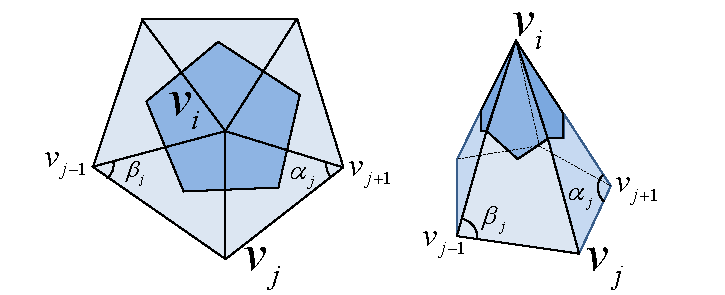
\includegraphics[width=1\textwidth]{resources/figs/voronoi_region}

\caption{\label{fig:voronoi_region}Area of the Voronoi region around $v_{i}$
in dark blue.$v_{j}$ belong to the first neighborhood around $v_{i}$.
$\alpha_{j}$ and $\beta_{j}$ opposite angles to edge $\protect\overrightarrow{v_{j}-v_{i}}$. }
\end{figure}


If the gradient in equation \ref{eq:eq_gradient_voronoi_area} is
normalized by the total area of the 1-ring neighborhood around $v_{i}$,
the \textsl{discrete mean curvature normal} of a surface $S$ is obtained,
as shown in equation \ref{eq:discrete_mean_curvature_normal}.

\noindent 
\begin{equation}
2\kappa\mathbf{n}=\frac{\nabla A}{A}\label{eq:discrete_mean_curvature_normal}
\end{equation}



\section{Laplace Beltrami Operator}

The \textit{Laplace Beltrami operator} LBO noted as $\Delta$ is used
for measuring the mean curvature normal to the Surface $S$ \cite{Pinkall1993}.

\noindent 
\begin{equation}
\Delta_{\mbox{S}}=2\kappa\mathbf{n}\label{eq:def_LBO}
\end{equation}



\chapter{Proposed Laplacian Operator\label{sec:Proposed-Method}}

This thesis propose an original extension of the Laplace Beltrami
operator for hybrid quad/triangle meshes, mixing arbitrary types of
meshes, exploiting the basic geometrical relationships and ensuring
algorithm convergence.

With the use of the proposed Laplacian Operator this work show succesful
uses in: Smoothing, Enhancing, Smooth Subdivision, Deformation, Sculpting,
and Skeletonization. 


\section{Proposed Laplace Beltrami Operator for Hybrid Quad/Triangle Meshes
TQLBO\label{sub:Laplace-Beltrami-operator}}

Given a mesh $M=\left(V,Q,T\right)$, with vertices $V$, quads $Q$,
triangles $T$. The area of $1$-ring neighborhood $A\left(v_{i}\right)$
corresponds to a sum of the areas of the quad faces $A\left(Q_{i}\right)$
and the areas of the triangular faces $\ensuremath{A\left(T_{i}\right)}$
adjacent to vertex $\ensuremath{v_{i}}$.

\noindent \begin{center}
$A\left(v_{i}\right)=A\left(Q_{i}\right)+A\left(T_{i}\right)$ 
\par\end{center}

\begin{figure}[H]
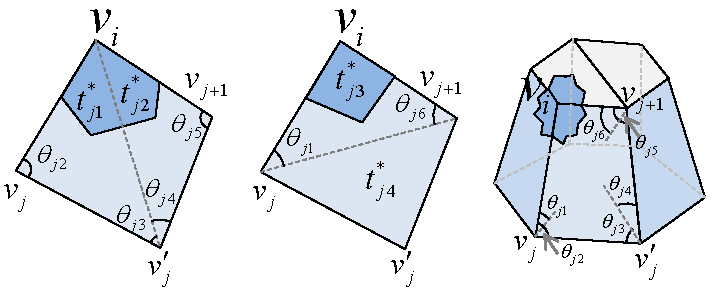
\includegraphics[width=1\columnwidth]{resources/figs/quad_xiong}

\caption{\label{fig:quad_xiong}$t_{j1}^{*}\equiv\vartriangle v_{i}v_{j}v_{j}^{\prime},\, t_{j2}^{*}\equiv\vartriangle v_{i}v_{j}^{\prime}v_{j+1},\, t_{j3}^{*}\equiv\vartriangle v_{i}v_{j}v_{j+1}$
Triangulations of the quad with common vertex $v_{i}$ proposed by
{[}Xiong 2011{]} to define Mean LBO.}
\end{figure}


Applying the mean average area, according to Xiong et. al. \cite{Xiong2011},
from all possible triangulations, as show in figure \ref{fig:quad_xiong},
the area for quads $\ensuremath{A\left(Q_{i}\right)}$ and triangles
$A\left(T_{i}\right)$ is.

\noindent \begin{center}
$A\left(v_{i}\right)=\frac{1}{2^{m}}\overset{m}{\underset{j=1}{\sum}}2^{m-1}A\left(q_{j}\right)+\overset{r}{\underset{k=1}{\sum}}A\left(t_{k}\right)$ 
\par\end{center}

Where $q_{1},q_{2},...,q_{j},...,q_{m}\in Q_{i}$ are quads adjacent
to $v_{i}$, and $t_{1},t_{2},...,t_{k},...,t_{r}\in T_{i}$ are triangles
adjacent to $v_{i}$.

Applying triangulations of the quad with common vertex $v_{i}$ proposed
by \cite{Xiong2011}.

\noindent 
\begin{equation}
A\left(v_{i}\right)=\frac{1}{2}\overset{m}{\underset{j=1}{\sum}}\left[A\left(t_{j1}^{*}\right)+A\left(t_{j2}^{*}\right)+A\left(t_{j3}^{*}\right)\right]+\overset{r}{\underset{k=1}{\sum}}A\left(t_{k}\right)\label{eq:area_1_ring_triangles_quads}
\end{equation}


Applying the gradient operator to (\ref{eq:area_1_ring_triangles_quads}).

\noindent {\small 
\begin{equation}
\nabla A\left(v_{i}\right)=\frac{1}{2}\overset{m}{\underset{j=1}{\sum}}\left[\nabla A\left(t_{j1}^{*}\right)+\nabla A\left(t_{j2}^{*}\right)+\nabla A\left(t_{j3}^{*}\right)\right]+\overset{r}{\underset{k=1}{\sum}}\nabla A\left(t_{k}\right)\label{eq:EqGrad}
\end{equation}
}{\small \par}

According to (\ref{eq:eq_gradient_voronoi_area}), we have.

\noindent \begin{center}
$\nabla A\left(t_{j1}^{*}\right)=\frac{\cot\theta_{j3}\left(v_{j}-v_{i}\right)+\cot\theta_{j2}\left(v_{j}^{\prime}-v_{i}\right)}{2}$ 
\par\end{center}

\noindent \begin{center}
$\nabla A\left(t_{j2}^{*}\right)=\frac{\cot\theta_{j5}\left(v_{j}^{\prime}-v_{i}\right)+\cot\theta_{j4}\left(v_{j+1}-v_{i}\right)}{2}$ 
\par\end{center}

\noindent \begin{center}
$\nabla A\left(t_{j3}^{*}\right)=\frac{\cot\theta_{j6}\left(v_{j}-v_{i}\right)+\cot\theta_{j1}\left(v_{j+1}-v_{i}\right)}{2}$ 
\par\end{center}

\noindent \begin{center}
$\nabla A\left(t_{k}\right)=\frac{\cot\alpha_{k}\left(v_{k}-v_{i}\right)+\cot\beta_{k+1}\left(v_{k+1}-v_{i}\right)}{2}$ 
\par\end{center}

Triangle and quad configurations of the 1-ring neighborhood faces,
adjacent to $v_{i}$, can be simplified to five cases, as shown in
figure \ref{fig:LBO-basic-5-TQ}.

\begin{figure}[H]
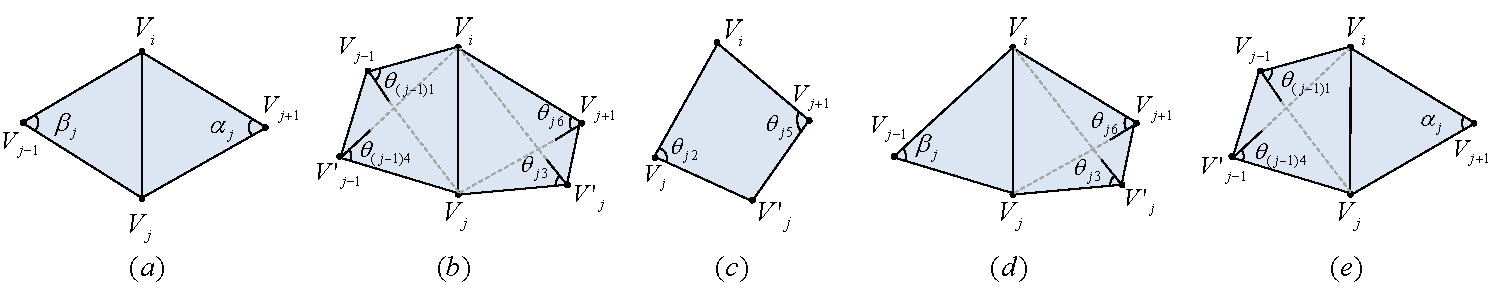
\includegraphics[width=1\textwidth]{resources/figs/beltrami}

\caption{\label{fig:LBO-basic-5-TQ}The 5 basic triangle-quad cases with common
vertex $V_{i}$ and the relationship with $V_{j}$ and $V_{j}^{\prime}$.
(a) Two triangles {[}Desbrun 1999{]}. (b) (c) Two quads and one quad
{[}Xiong 2011{]}. (d) (e) Triangles and quads (TQLBO) our contribution.}


\end{figure}


According to equation (\ref{eq:discrete_mean_curvature_normal}),
(\ref{eq:def_LBO}), and five simple cases defined in figure \ref{fig:LBO-basic-5-TQ}
the TQLBO (Triangle-Quad LBO) of $v_{i}$ is.

\noindent 
\begin{equation}
\triangle_{S}\left(v_{i}\right)=2\kappa\mathbf{n}=\frac{\nabla A}{A}=\underset{v_{j}\in N_{1}\left(v_{i}\right)}{\frac{1}{2A}\sum}w_{ij}\left(v_{j}-v_{i}\right)
\end{equation}


\noindent {\small where
\begin{equation}
w_{ij}=\begin{cases}
\left(\cot\alpha_{j}+\cot\beta_{j}\right) & \mbox{case }\mathit{a.}\\
\frac{1}{2}\left(\cot\theta_{\left(j-1\right)1}+\cot\theta_{\left(j-1\right)4}+\cot\theta_{j3}+\cot\theta_{j6}\right) & \mbox{case \ensuremath{\mathit{b}}.}\\
\left(\cot\theta_{j2}+\cot\theta_{j5}\right) & \mbox{case \ensuremath{\mathit{c}}.}\\
\frac{1}{2}\left(\cot\theta_{j3}+\cot\theta_{j6}\right)+\cot\beta_{j} & \mbox{case \ensuremath{\mathit{d}}.}\\
\frac{1}{2}\left(\cot\theta_{\left(j-1\right)1}+\cot\theta_{\left(j-1\right)4}\right)+\cot\alpha_{j} & \mbox{case \ensuremath{\mathit{e}}.}
\end{cases}\label{eq:TQLBO_wij}
\end{equation}
}{\small \par}

We define a Laplacian operator as a matrix equation

\noindent 
\begin{equation}
L\left(i,j\right)=\begin{cases}
-\frac{1}{2A_{i}}w_{ij} & \mbox{if }j\in N\left(v_{i}\right)\\
\frac{1}{2A_{i}}\underset{j\in N\left(v_{i}\right)}{\sum}w_{ij} & \mbox{if }i=j\\
0 & \mbox{otherwise}
\end{cases}\label{eq:TQLBO_Simple_Matrix}
\end{equation}


Where $L$ is a $n\times n$ matrix, $n$ is the number of vertices
of a given mesh $M$, $w_{ij}$ is the TQLBO defined in equation (\ref{eq:TQLBO_wij}),
$N\left(v_{i}\right)$ is the 1-ring neighborhood with shared face
to $v_{i}$, $A_{i}$ is the ring area around $v_{i}$.

Normalized version of the TQLBO as a matrix equation

\noindent 
\begin{equation}
L\left(i,j\right)=\begin{cases}
-\frac{w_{ij}}{\underset{j\in N\left(v_{i}\right)}{\sum}w_{ij}} & \mbox{if }j\in N\left(v_{i}\right)\\
\delta_{ij} & \mbox{otherwise}
\end{cases}\label{eq:TQLBO-Normalized_Matrix}
\end{equation}


Where $\delta_{ij}$ being the Kronecker delta function.


\section{Mesh Smoothing\label{sub:Laplacian-Smooth}}

Computer objects, reconstructed from the real world, are usually noisy.
A common way to attenueate noise in a polygonal mesh is through a
diffusion process \cite{Taubin1995,Desbrun1999}. Laplacian smooth
techniques over a diffusion process allow a proper noise reduction
on the mesh surface with minimal shape changes, while still preserving
a desirable geometry as well as the original shape. The simple idea
is that the vertices are moved in the direction of the Laplacian when
we use the contangent version the vertices are moved in the direction
of the curvature flow. The complexity of Laplacian smoothing can be
linear in time and space with a fast convergence and the diffussion
proccess can attenuate noise with only one iteration due the sparseness
of the laplacian operator.

\noindent 
\begin{equation}
\frac{\partial V}{\partial t}=\lambda L\left(V\right)\label{eq:diffusion_process}
\end{equation}


Where L is the Laplacian matrix defined in equation \ref{eq:TQLBO-Normalized_Matrix}
for meshes with regular sampling, and equation \ref{eq:TQLBO_Simple_Matrix}
for meshes composed by triangles or quads with differents size or
irregular sampling. $\lambda$ is a scalar that control the diffussion
proccess, and smoothing factor.

The equation \ref{eq:diffusion_process} can be linearly approximated
using implicit integration with a Laplacian Operator version of TQLBO,
the use of implicit integration permit the system to be more stability.

\begin{equation}
\left(I-\lambda\partial tL\right)V^{n+1}=V^{n}\label{eq:LaplacianSmoothLinearEquationSystem}
\end{equation}



\section{The Shape Inflation\label{sub:Curvature-Enhancing}}

\begin{figure}[H]
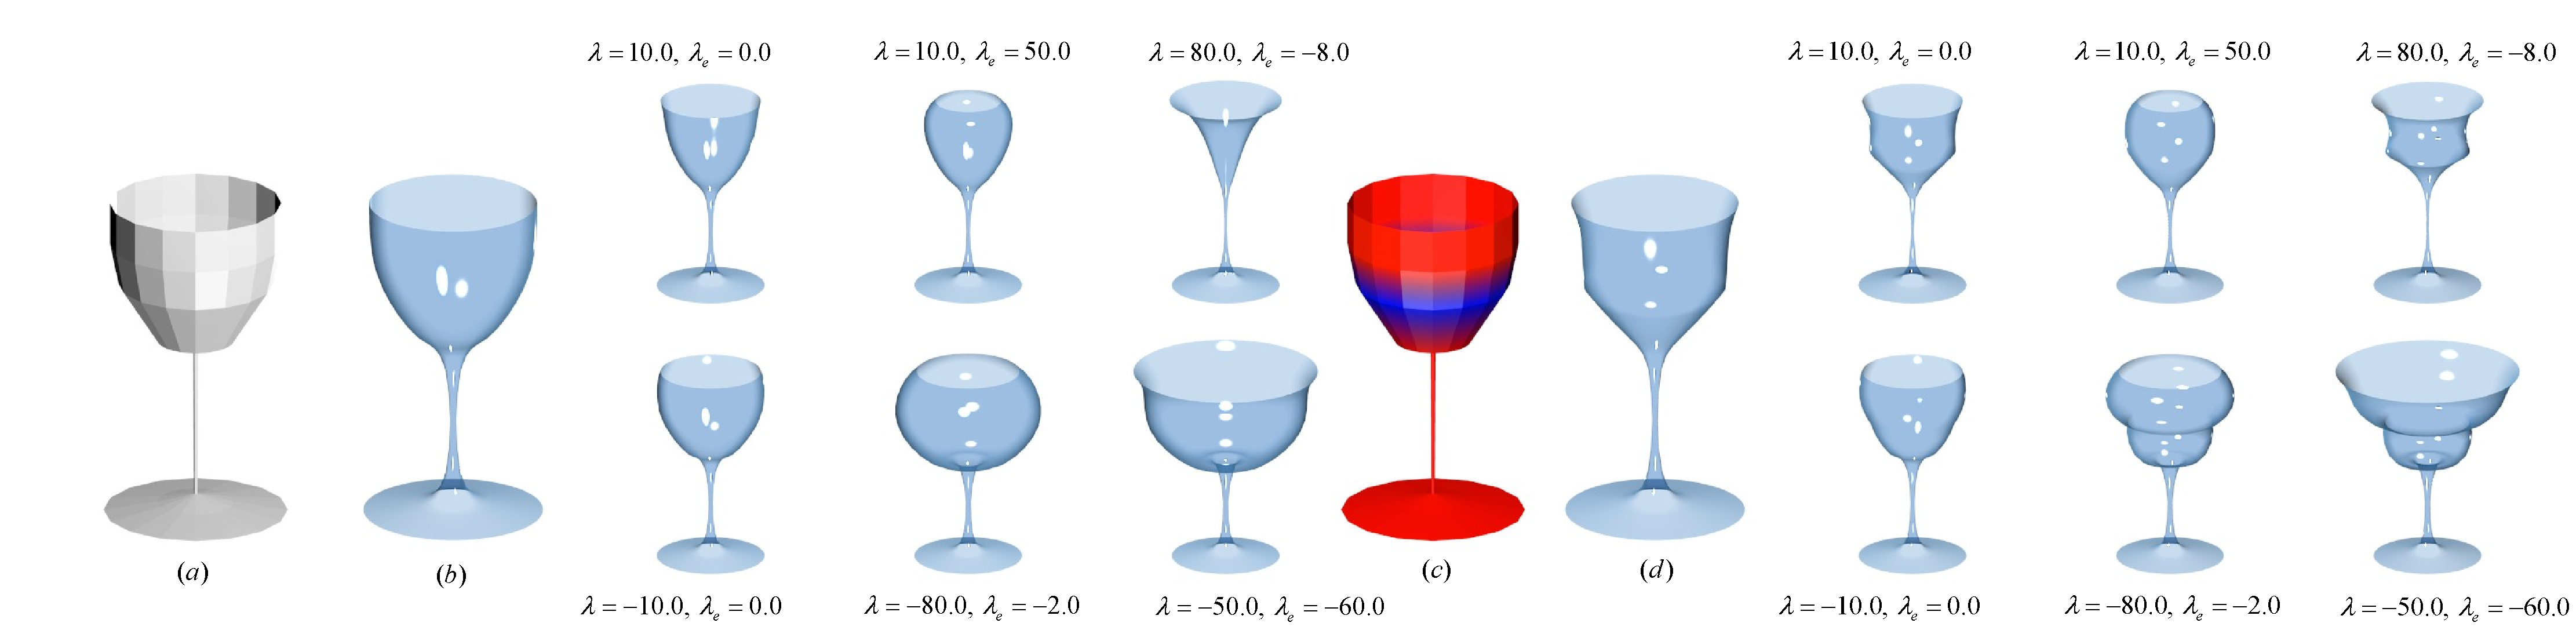
\includegraphics[width=1\textwidth]{resources/figs/teaser_cup}

\caption{\label{fig:Subdivision-Cups} Family of cups generated with our method,
from a coarse model (a), (c): the shape, obtained from the Catmull-Clark
Subdivision (b), (d), is inflated. Soft constraints, over the coarse
model, is drawn in red and blue (c).}
\end{figure}


This method exaggerates a shape using a Laplacian smoothing operator
in the reverse direction, i.e., the new shape is a modified version
in which those areas with larger curvature are magnified. The operator
amounts to a generator of a set of models which conserves the basic
silhouette of the original shape. In addition, the presented approach
can be easily mixed with traditional or uniform subdivision of surfaces. 

The shape is inflated by using the reverse direction of the curvature
flow, moving the vertices towards those mesh portions with larger
curvature. A standard diffusion process is applied:

\noindent \begin{center}
$\frac{\partial V}{\partial t}=\lambda L\left(V\right)$ 
\par\end{center}

To solve this equation, implicit integration is used as well as a
normalized version of TQLBO matrix.

\noindent 
\begin{equation}
\left(I-\left|\lambda dt\right|W_{p}L\right)V^{\prime}=V^{t}\label{eq:Lineal_System_with_wp}
\end{equation}


\noindent \begin{center}
$V^{t+1}=V^{t}+\mbox{sign}\left(\lambda\right)\left(V^{\prime}-V^{t}\right)$ 
\par\end{center}

The vertices $V^{t+1}$ are inflated, along their reverse curvature
direction, by solving the linear system: $Ax=b$, where $A=I-\left|\lambda dt\right|W_{p}L$,~
$L$ is the Normalized TQLBO defined in the equation (\ref{eq:TQLBO-Normalized_Matrix}),
$x=V^{\prime}$ are the smoothing vertices, $b=V^{t}$ are the actual
vertices positions, $W_{p}$ is a diagonal matrix with vertex weights,
and $\lambda dt$ is the inflate factor that supports negative and
positive values: negative for inflation and positive for smoothing.

The method was devised to use with weighted vertex groups, which specify
the final shape inflation of the solution, meaning $0$ as no changes
and 1 when a maximal change is applied. The weights modify the influence
zones, where the Laplacian is applied, as shown in equation \ref{eq:Lineal_System_with_wp}.
Interestingly, the generated family of shapes may change substantially
with the weights of specific control points.

The curvature cannot be calculted at the boundary of the meshes that
are not closed, for that reason we use the scale-dependent operator
proposed by Desbrun et al. \cite{Desbrun1999}, the inflation factor
for boundary is represented by $\lambda_{e}$.

The model volume increases as the lambda is larger and negative, this
can be counteracted with a simple volume preservation. However, the
mesh may suffer large displacements when $\lambda<-1.0$ or after
multiple iterations. A simple volume conservation algorithm is: If
$v_{i}^{t+1}$ is a mesh vertex of $V^{t+1}$ in the $t+1$ iteration,
we define $\overline{v}$ as:

\noindent \begin{center}
$\overline{v}=\frac{1}{n}\underset{v_{i}\in V}{\sum}v_{i}$, 
\par\end{center}

$\overline{v}$ is the mesh center, $vol_{ini}$ is an initial volume,
and $vol_{t+1}$ is the volume at the iteration $t+1$, then the scale
factor.

\noindent \begin{center}
$\beta=\left(\frac{vol_{ini}}{vol_{t+1}}\right)^{\frac{1}{3}}$ 
\par\end{center}

allows to scale the vertices to:

\noindent \begin{center}
$v_{i\, new}^{t+1}=\beta\left(v_{i}^{t+1}-\overline{v}\right)+\overline{v}$ 
\par\end{center}

The shape inflation use a negative curvature flow that is an unstable
process when performing many iterations, however, our method uses
less than 3 iterations to get good results, and with 3 iterations
or less the method behaves stable.


\section{Sculpting\label{sub:Sculpting}}

A new sculpting brush is herein proposed and aims to inflate the shape,
magnifying the shape curvatures of a polygon mesh in real time. This
brush works properly with the stroke method \textsl{Drag Dot}, allowing
to pre-visualize the model changes before the mouse is released. Also,
it allows to move the mouse along the model to match the shape zone
which is supposed to be inflated.

Brushes that perform a similar inflation can introduce mesh distortions
or produce mesh self-intersections, provided these brushes only move
the vertices along the normal without any global information. In contrast,
the present method searches for a proper inflation while preserving
the global curvature, retaining the original shape and main model
features. In addition, this method simplifies the work required for
the inflation since it needs not different brushes for inflating,
softening or styling. The inflated brush can make all these operation
in a single step. Real-time brushes require the Laplacian matrix is
constructed with the vertices that are within the sphere radius defined
by the user, reducing the matrix to be processed, the center of this
sphere depending on the place where the user clicks on the canvas
and the three-dimensional mesh placed where the click is projected.
Special handling is required for the boundary vertices with neighbors
that are not within the brush radius: these vertices are marked as
boundary and the curvature is not there calculated, but they must
be included in the matrix so that every vertex has their corresponding
neighbors within the selection. The sculpting Laplacian matrix reads
as.

\noindent \begin{center}
$L\left(i,j\right)=\begin{cases}
-\frac{w_{ij}}{\underset{j\in N\left(v_{i}\right)}{\sum}w_{ij}} & \mbox{if }\left\Vert v_{i}-u\right\Vert <r\wedge\left\Vert v_{j}-u\right\Vert <r\\
0 & \mbox{if }\left\Vert v_{i}-u\right\Vert <r\wedge\left\Vert v_{j}-u\right\Vert \geq r\\
\delta_{ij} & \mbox{otherwise}
\end{cases}$ 
\par\end{center}

Where $v_{j}\in N\left(v_{i}\right)$, $u$ is the sphere center of
radius $r$. The matrices should remove rows and columns of vertices
that are not within the radius.


\section{Laplacian Deform\label{sub:Laplacian-Deform}}

The Laplacian deform allows to pose a mesh while preserving geometric
details of the surface. This method allows to defines a set of anchor
vertices, and then moves some of them around. The system keeps the
rest of the anchor vertices in fixed positions, and calculates the
best possible locations of all the remaining vertices to preserve
the original geometric details.

This thesis adapt the method proposed by Sorkine \cite{Sorkine2004}
for mesh deformations, delete the use of static vertices and allow
application of this system in hybrid meshes composes by triangles
and quads with the TQLBO proposed.

This method captures the geometric details using a differential coordinates
representations. The differential coordinates captures the local geometric
information (curvature and direction) of the vertex based on its neighbors
how show in figure \ref{fig:DifferentialCoor}.

\begin{figure}
\noindent \begin{centering}
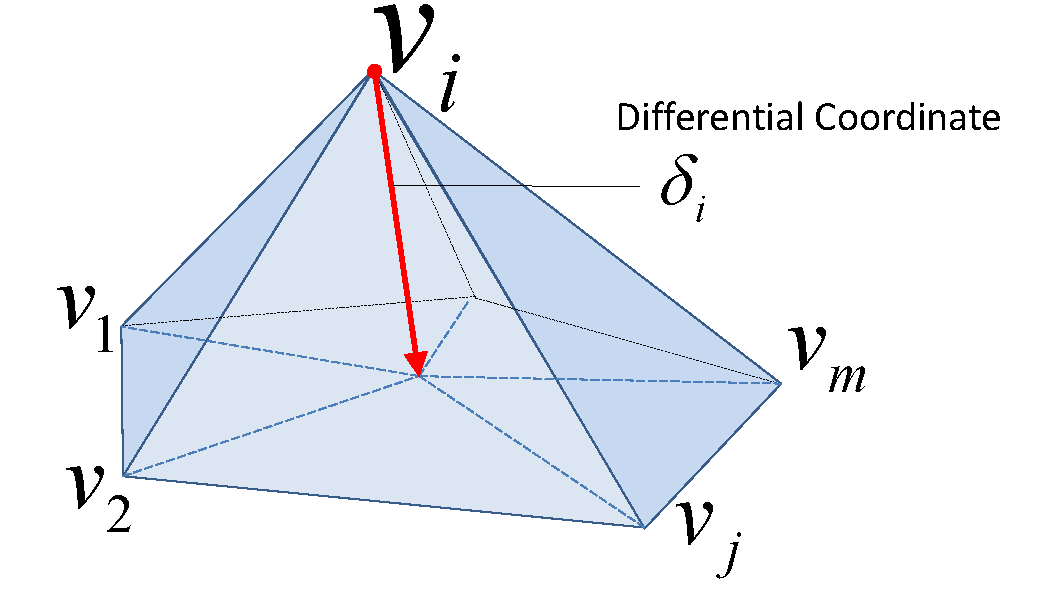
\includegraphics[width=0.7\columnwidth]{resources/figs/DifferentialCoordinates}
\par\end{centering}

\caption{\label{fig:DifferentialCoor} Difference between $v_{i}$ and the
center of mass of its neighboors $v_{1},...,v$.}
\end{figure}


\begin{equation}
\delta_{i}=\overset{m}{\underset{j=1}{\sum}}w_{ij}\left(v_{i}-v_{j}\right)\label{eq:DifferentialCoordinate}
\end{equation}


Where $\delta_{i}$ is the differential coordinate for vertex $v_{i}$.
The $v_{j}$ are the inmediate neighoors of $v_{i}$, and $w_{ij}$
is the weigth betwen vertex $v_{i}$ and $v_{j}$ defined in equation
\ref{eq:TQLBO_wij} that is TQLBO.

Then the linear systems for find the new pose of a mesh is.

\begin{equation}
\begin{bmatrix}w_{l}L\\
W_{c}
\end{bmatrix}X=\begin{bmatrix}\delta\\
W_{c}C
\end{bmatrix}\label{eq:LaplacianDefomSystem}
\end{equation}


Where $w_{l}$ is the weigth for Laplacian Matrix $L$, the Laplacian
matrix $L$ was defined in equation \ref{eq:TQLBO_Simple_Matrix}
. $Wc$ is a matrix that containts ones int the indexes of anchors
vertices. $C$ is a vector with coordinates of anchors vertices after
several transformatios. $\delta$ are the differential coordinates
defined in equation \ref{eq:DifferentialCoordinate}.


\section{Subdivision surfaces\label{sub:Subdivision-surfaces}}

The Catmull-Clark subdivision transformation is used to smooth a surface,
as the limit of a sequence of subdivision steps \cite{Stam1998}.
This process is governed by a B-spline curve \cite{Loop1987}, performing
a recursive subdivision transformation that refines the model into
a linear interpolation that approximates a smooth surface. The model
smoothness is automatically guaranteed \cite{DeRose1998}.

\begin{figure}[H]
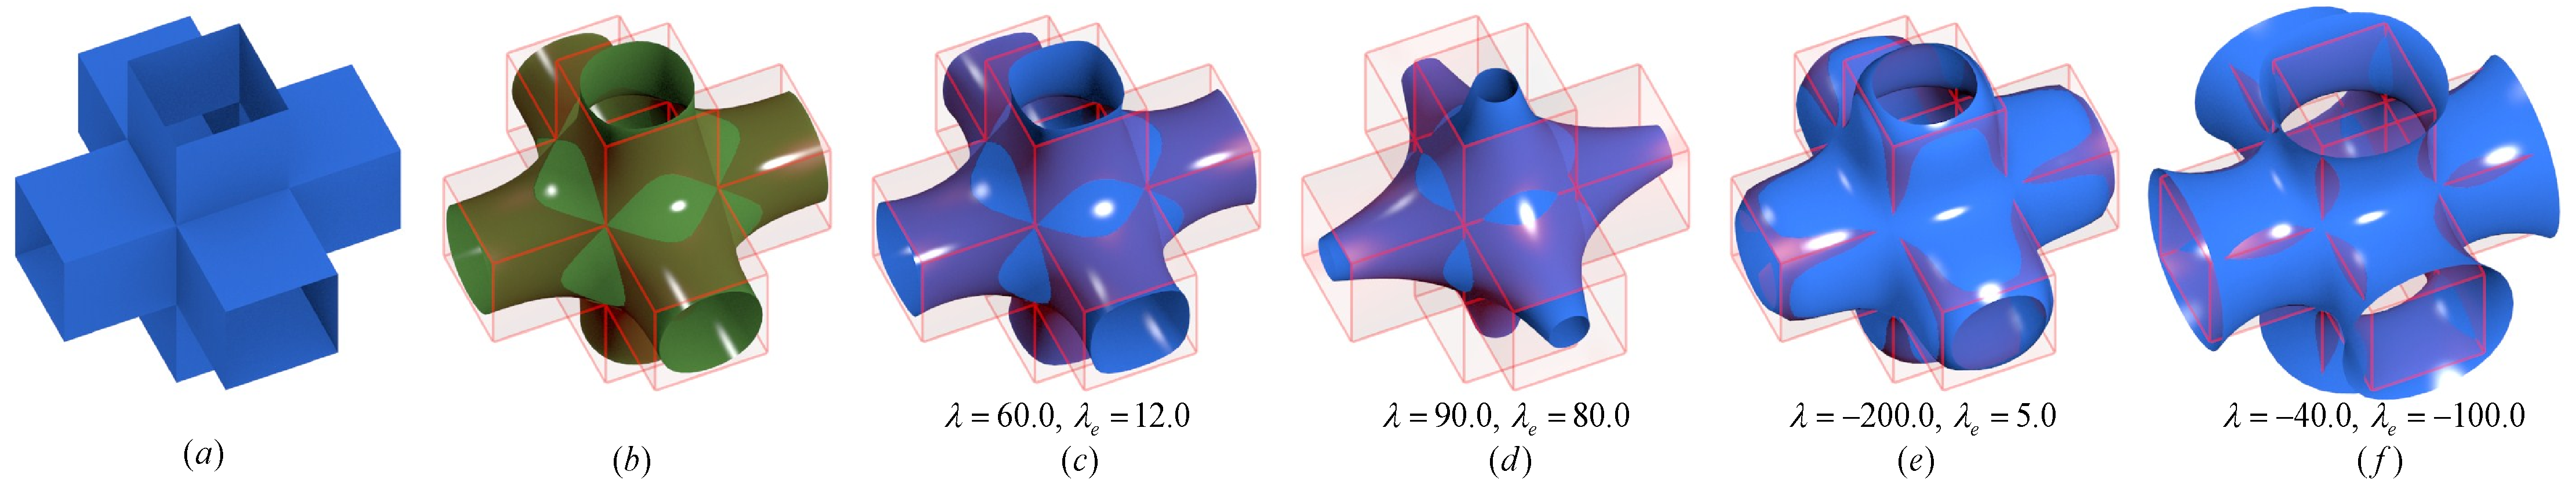
\includegraphics[width=1\textwidth]{resources/figs/cruz_lambda4}

\caption{\label{fig:Catmull_Clark}(a) Original Model, (b) Model with Catmull-Clark
Subdivision. Models with Laplacian smoothing: (c) and (d). Models
with a first Laplacian filtering $\lambda=60.0$, $\lambda_{e}=12.0$
and before applying shape inflation: (e) and (f).}
\end{figure}


Catmull-Clark subdivision surface methods generate smooth and continuous
models from a coarse model and produce quick results because of the
simplicity of implementation. Nevertheless, changes to the global
curvature are hardly implantable. The Catmull-Clark subdivision surfaces
together with shape inflation can easily generate families of shapes
by changing a single parameter, allowing to handle a model with very
few vertices. In practice, this would allow an artist to choose a
model from a similar set of options that would meet his/her needs
without having to change each of the control vertices. Likewise, the
presented method allows the use of vertex weight paint over the control
points. The weights can be applied to a coarse model, followed by
a Catmull-Clark subdivision where weights are interpolated, producing
weights with smooth changes in the influence zones, as shown in figure
\ref{fig:Subdivision-Cups}.c.

In equation \ref{eq:Lineal_System_with_wp}, $W_{p}$ is a diagonal
matrix with weights corresponding to each vertex. Weights at each
vertex produce a different solution so that the matrix must be placed
in the diffusion equation since families that are generated may change
substantially with weighted of specific control points.


\section{Skeleton Extraction}

Skelton extraction reduces the dimensionality and represents a three-dimensional
object as a uni-dimensional structure \cite{Cornea2007}.

The skeleton extraction use the natural shrink produced by the laplacian
smoothing \cite{Meyer2003}, to contratc iteratively the mesh until
the volume inside the surface is near to zero (see figure \ref{fig:MeshContracted}).
The method stretch the shrink mesh to warranty that object preservers
the best at posibble the original topology with the use of attraction
constraint \cite{Au2008}.

\begin{figure}[H]
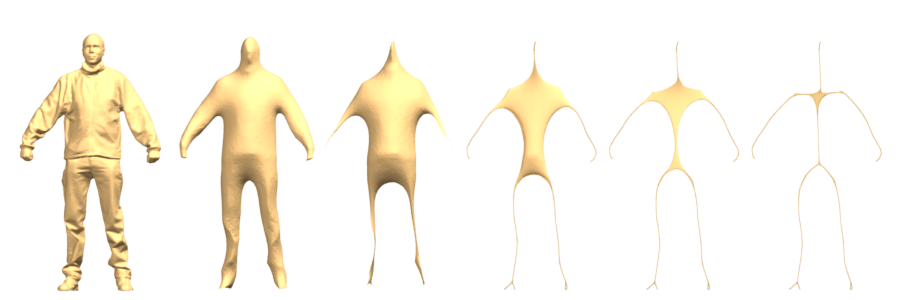
\includegraphics[width=1\textwidth]{resources/figs/contraccion}

\caption{\label{fig:MeshContracted}From left to right iterative mesh contraction.}
\end{figure}


The laplacian smooth proccess move the vertices in the direction of
the Laplacian, if cotangent laplacian operator is used, the vertices
move in the direction of minimal surface \cite{Pinkall1993} following
the curvature flow of the mesh surface.

In the work of Au \cite{Au2008} is proposed the next system of equation
to iteratively contratc the mesh until a skeleton.

\begin{equation}
\left[\begin{array}{c}
W_{L}L\\
W_{H}
\end{array}\right]X_{t+1}=\left[\begin{array}{c}
0\\
W_{H}X_{t}
\end{array}\right]\label{eq:SkeletonExtraction}
\end{equation}


where $L$ is the Laplacian matrix describe in equation \ref{eq:TQLBO_Simple_Matrix},
$W_{L}$ is the factor for smoothing, $W_{H}$ is the factor for attraction
constraint.

$W_{L}$ and $W_{H}$ are changing in every iteration. The contraction
and smoothing constraint $W_{L}^{t+1}=S_{L}W_{L}^{t}$ with $S_{L}=2.0$.
The attraction constraint $W_{H,i}^{t+1}=W_{H,i}^{0}\sqrt{\frac{A_{i}^{0}}{A_{i}^{t}}}$.

$A_{i}^{t}$ y $A_{i}^{0}$ are the current area and initial aerea
of the ring surrounding $x_{i}$.

In this thesis an additional constraint is proposed which seeks the
vertices and the skeleton does not shrink, to eliminate the need to
adjust the final skeleton taking each skeleton node and move to the
center of your local mesh region.

The basic idea is move the vertices along of the normal line estimated
on every vertex based on the avergage of the faces normals. 

\begin{figure}[H]
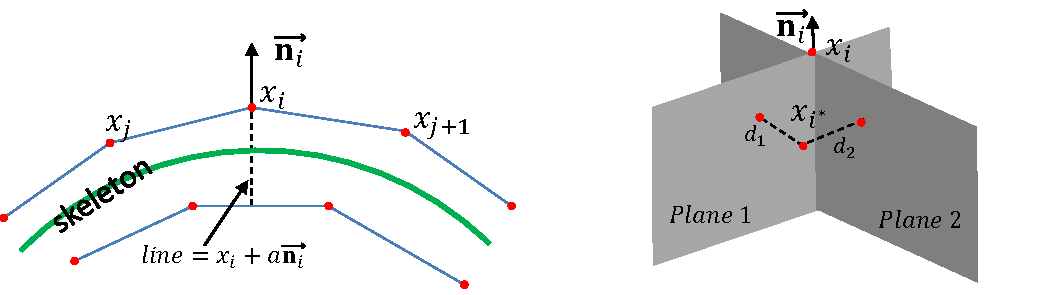
\includegraphics[width=1\textwidth]{resources/figs/LineConstraintSkeleton}

\caption{\label{fig:LineConstraint}Left: The vertex $x_{i}$ move along line
constraint. Right: the distance of vertex $x_{i}$ to plane 1 and
plane 2 when change the position in every iteration.}
\end{figure}


This line can be see as intersection of two planes (see figure \ref{fig:LineConstraint})
created with the information of the vertex $x_{i}$, the normal $\overrightarrow{\mathbf{n}_{i}}$
and neighboors $x_{j}$ of $x_{i}$. 

The equation of the plane.

\noindent \begin{center}
$a\mathbf{x}+b_{0}\mathbf{y}+c_{0}\mathbf{z}+d_{0}=0$
\par\end{center}

There is varios methods to build a equation of the plane based on
three non-collinear points, we choose this three points based on vertex
$x_{i}$, the normal $\overrightarrow{\mathbf{n}_{i}}$ and neighboors
$x_{j}$ of $x_{i}$.

$P_{1}=x_{i}$, $P_{2}=x_{j}$ when $x_{j}\in Neighboors\left(x_{i}\right)$
and $P_{3}=P_{1}-\overrightarrow{\mathbf{n}_{i}}$.

To build a equation plane only need three non-collinear points $\left\{ P_{1},P_{2},P_{3}\right\} $
and solve the next systems of equations for variables $a,b,c$.

\noindent \begin{center}
$\begin{array}{c}
ax_{1}+by_{1}+cz_{1}+d=0\\
ax_{2}+by_{2}+cz_{2}+d=0\\
ax_{3}+by_{3}+cz_{3}+d=0
\end{array}$
\par\end{center}

The distance of point $P_{0}=\{x_{0},y_{0},z_{0}\}$ to a plane $\Pi=a\mathbf{x}+b_{0}\mathbf{y}+c_{0}\mathbf{z}+d_{0}$.

\noindent \begin{center}
$\left|\Pi-P_{0}\right|=\frac{\left|ax_{0}+by_{0}+cz_{0}+d\right|}{\sqrt{a^{2}+b^{2}+c^{2}}}$
\par\end{center}

In the equation above, every point $P_{0}=\{x_{0},y_{0},z_{0}\}$
that belong to plane made the equation zero. If the point $P_{0}$
is not in the plane the value of the equation of the plane change,
and the absolute value is increased if $P_{0}$ is more distant of
the plane. Let us use this simple relation to build a valid constraint
that can be put in the form of linear equation $Ax=B$. Where $A$
is the matrix with values $\begin{vmatrix}a & b & c\end{vmatrix}$
the $x$ value correspond to every vertex in mesh $\{x_{0},y_{0},z_{0}\}$
and $B$ correspond to $d$ value of the plane equation. How the linear
system presented in equation \ref{eq:SkeletonExtraction} don't has
a unique solution, the system solve it in the least-squares sense.
With the new constraint the system then try to minimize the distance
betwen the new vertex positions and the two planes. 

The new system of equations proposed

\begin{equation}
\left[\begin{array}{c}
W_{L}L\\
W_{H}\\
W_{D}\Pi_{1}\\
W_{D}\Pi_{2}
\end{array}\right]X_{t+1}=\left[\begin{array}{c}
0\\
W_{H}X_{t}\\
-D_{1}\\
-D_{2}
\end{array}\right]\label{eq:SkeletonExtractionDistance}
\end{equation}


where $W_{D}$ is the weigth to new constraints, that forced the vertices
to move along of the normal line of every vertex. $\Pi_{1}$ and $\Pi_{2}$
are matrix that contains $a,b,c$ values of the equation of the plane
for every vertex. $D_{1}$ and $D_{2}$ are the vector with $d$ values
of the equations of the planes for every vertex.


\chapter{Results\label{sec:Results}}

This chapter show the results of the Laplace Beltrami operator for
hybrid quad/triangle meshes with several example models (see figures
\ref{fig:Spectrum}, \ref{fig:Subdivision-Cups}, \ref{fig:Catmull_Clark},
\ref{fig:TQLBO_test}, \ref{fig:camello_enhanced}, \ref{fig:Sculpt_Brush},
\ref{fig:Performance-sculpt}, \ref{fig:(a)Monkey}, \ref{fig:Animated_Camell}).
It first show a comparisson of the Laplacian Operator in meshes composed
by triangles, by quads and hybrid meshes composed by triangles/quads.
Section \ref{sec:Customizing-Curvature-by} show the use of TQLBO
in applications of Shape Inflation and Subdivision Surfaces on normal
meshes and meshes change with isometric transformations. It Section
\ref{sec:Shape-Inflation-Brush} show a novel shape inflation brush
for sculpting systems that works in real time. It Section \ref{sec:Posing-Meshes-with}
show mesh deformations and posing applications using differential
coordinates defined with the TQLBO. It Section \ref{sec:Laplace-Operator-and}
discusses the differences betwen common version and normalized version
of the TQLBO. It Section \ref{sec:Performance-Testing-of} describe
a performance comparison of differents numericals solvers used to
solve a Laplacian linear equation system. Finally discusses some especific
technical aspect about the implementation of the TQLBO on several
computer systems at Section \ref{sec:Conclusion-and-future}.

Figure \ref{fig:TQLBO_test} shows the results when applying the Laplace
Beltrami Operator TQLBO of equation (\ref{eq:TQLBO_Simple_Matrix})
in a model with a simple subdivision. In column (c) the Laplacian
smoothing was applied to a model consisting of only quads. In column
(d) the model was converted to triangles and then the Laplacian smoothing
was applied. In column (e) the model was randomly converted from some
quads into triangles and then the Laplacian smoothing is applied,
showing similar results to those meshes composed only of triangles
or quads.

\begin{figure}[H]
\noindent \begin{centering}
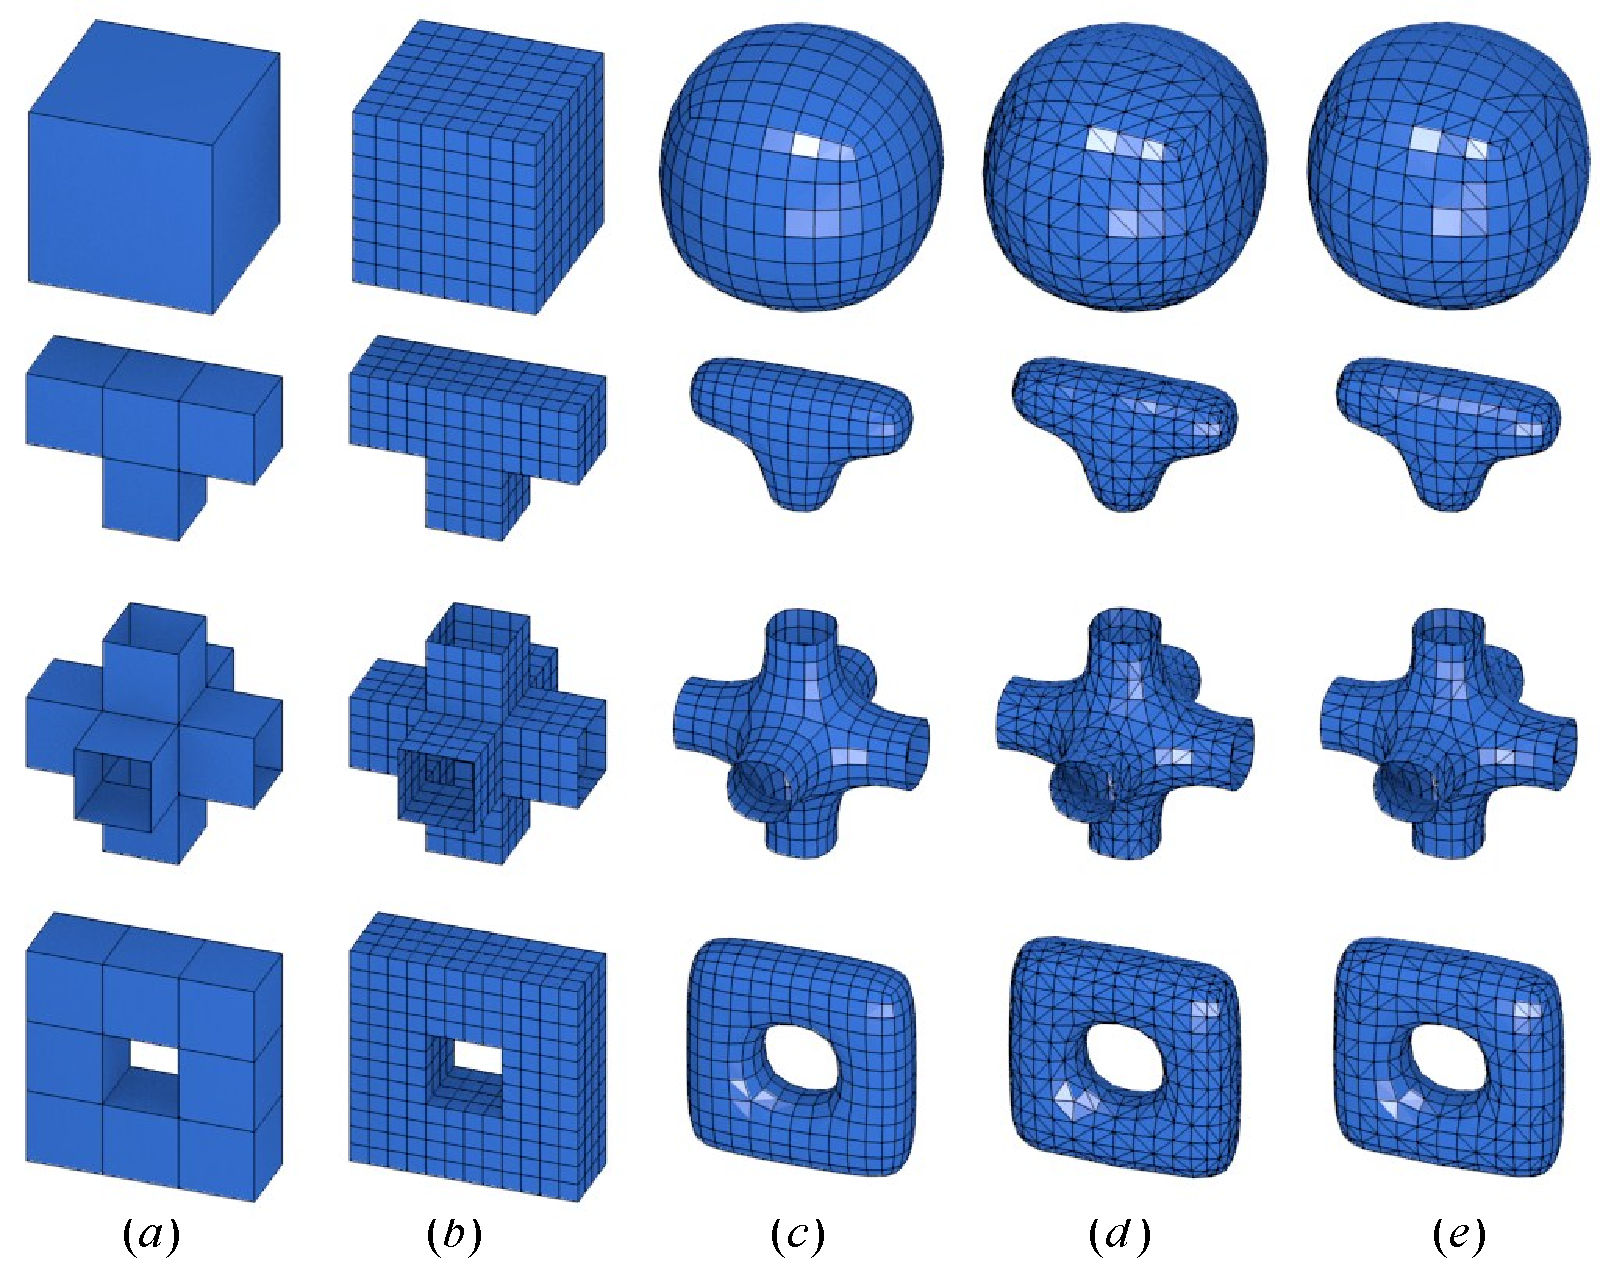
\includegraphics[height=0.5\textheight]{resources/figs/test_triangles_quads}
\par\end{centering}

\caption{\label{fig:TQLBO_test}(a) Original Model. (b) Simple subdivision.
(c), (d) (e) Laplacian smoothing with $\lambda=7$ and 2 iterations:
(c) for triangles, (d) for quads, (e) for triangles and quads random
chosen.}
\end{figure}



\section{Customizing Curvature by Shape Inflation.\label{sec:Customizing-Curvature-by}}

\begin{figure}[H]
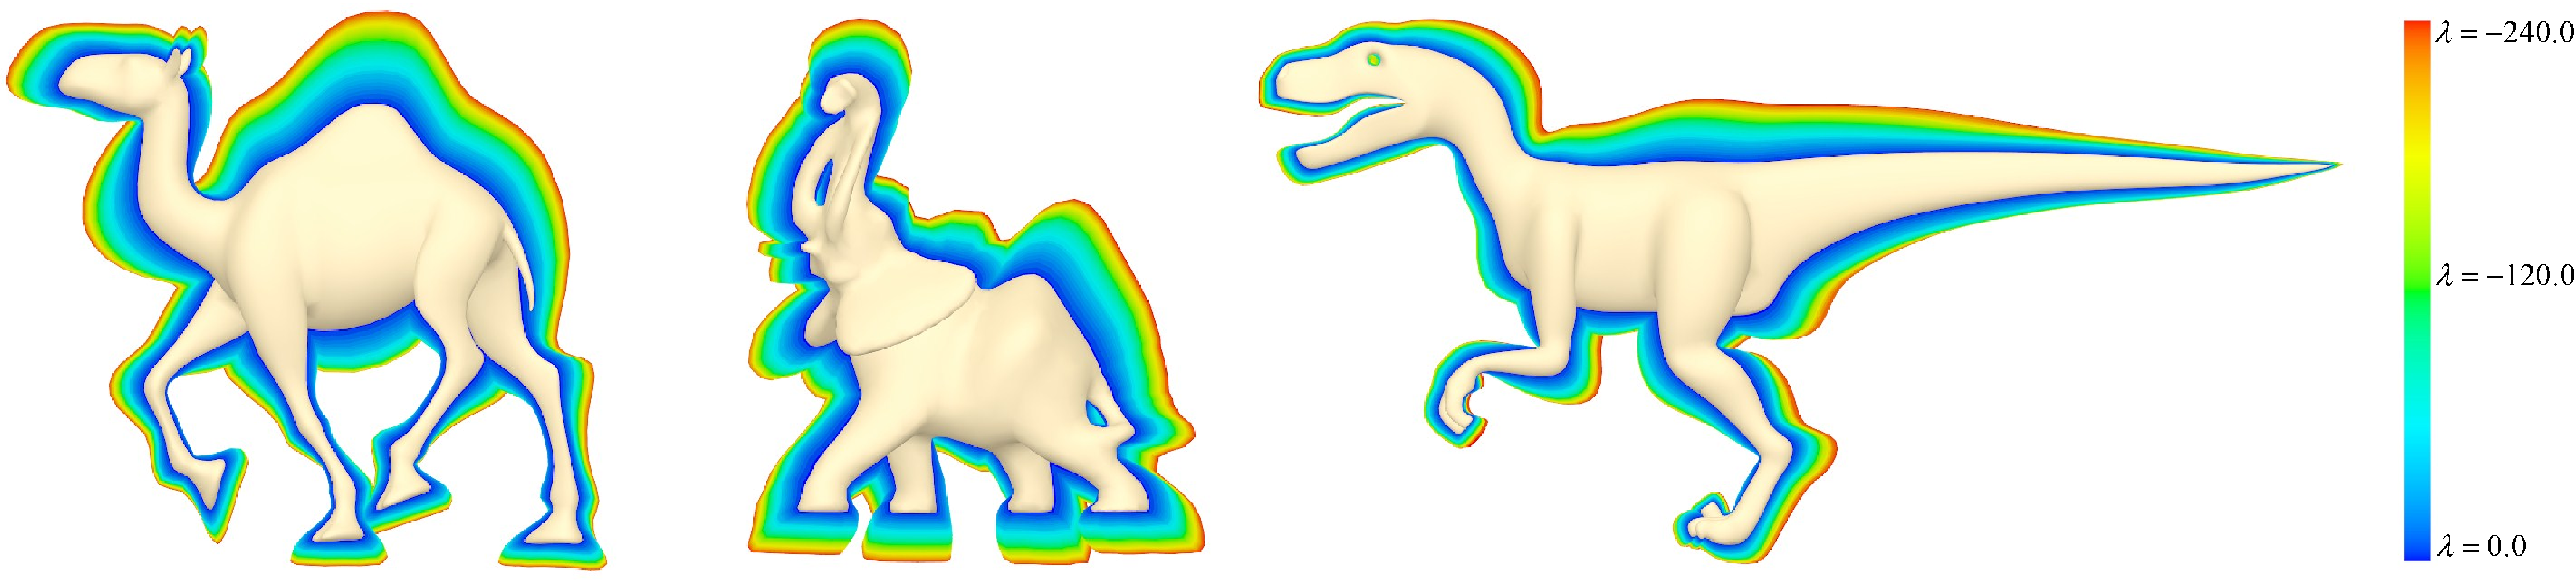
\includegraphics[width=1\textwidth]{resources/figs/spectrum}

\caption{\label{fig:Spectrum}A set of 48 successive shapes enhanced, from
$\lambda=0.0$ in blue to $\lambda=-240.0$ in red, with steps of
$-5.0$.}
\end{figure}


The shape inflation was assessed with TQLBO method on a PC with AMD
Quad-Core Processor @ 2.40 GHz and 8 GB RAM.

Methods using the Catmull-Clark subdivision surface and the inflation
allows to modify the curvature that is obtained with the process of
subdivision, as shown in figure \eqref{fig:Subdivision-Cups}. This
test used a coarse cup model, in which the subdivision was performed,
followed by a Laplacian smoothing and inflation. In figure \eqref{fig:Subdivision-Cups}.c,
\eqref{fig:Subdivision-Cups}.d shows also the use of weight vertex
groups over coarse models, with subdivision surfaces that allowed
to generate the weights for the new interpolated vertices. These new
weights were used for the inflation obtained on the 6 cups that are
at the right of the figure \eqref{fig:Subdivision-Cups}.d.

Laplacian smoothing applied with simple subdivision (see figure \ref{fig:Catmull_Clark}.b.)
may produce similar results to those obtained with Catmull-Clark (see
figure \ref{fig:Catmull_Clark}.c.), whose models are in average equal
triangles. The one obtained with the Laplacian smoothing is shown
in panel (c), (d) and those curvature modified versions are in (e)
and (f). As can be observed, different versions of the original sketch
can be obtained by parameterizing a single model value, a great advantage
of the presented method. Figure \ref{fig:camello_enhanced} shows
the generation of different versions of a camel according to the $\lambda$
parameter. In the top row, it is shown the shape inflation results,
as $\lambda$ becomes larger and negative, the resultant shape is
observed as if the model would inflate the more convex parts, as shown
in figure \ref{fig:Spectrum}. The larger the $\lambda$ parameter
the larger the model feature inflations. The bottom row of figure
\ref{fig:camello_enhanced} shows the use of weighted vertex groups,
specifying which areas will be inflated. On the left, the inflation
of the camel legs produces an organic aspect, notice that the border
is not distorted and smooth.

\begin{figure}[H]
\noindent \begin{centering}
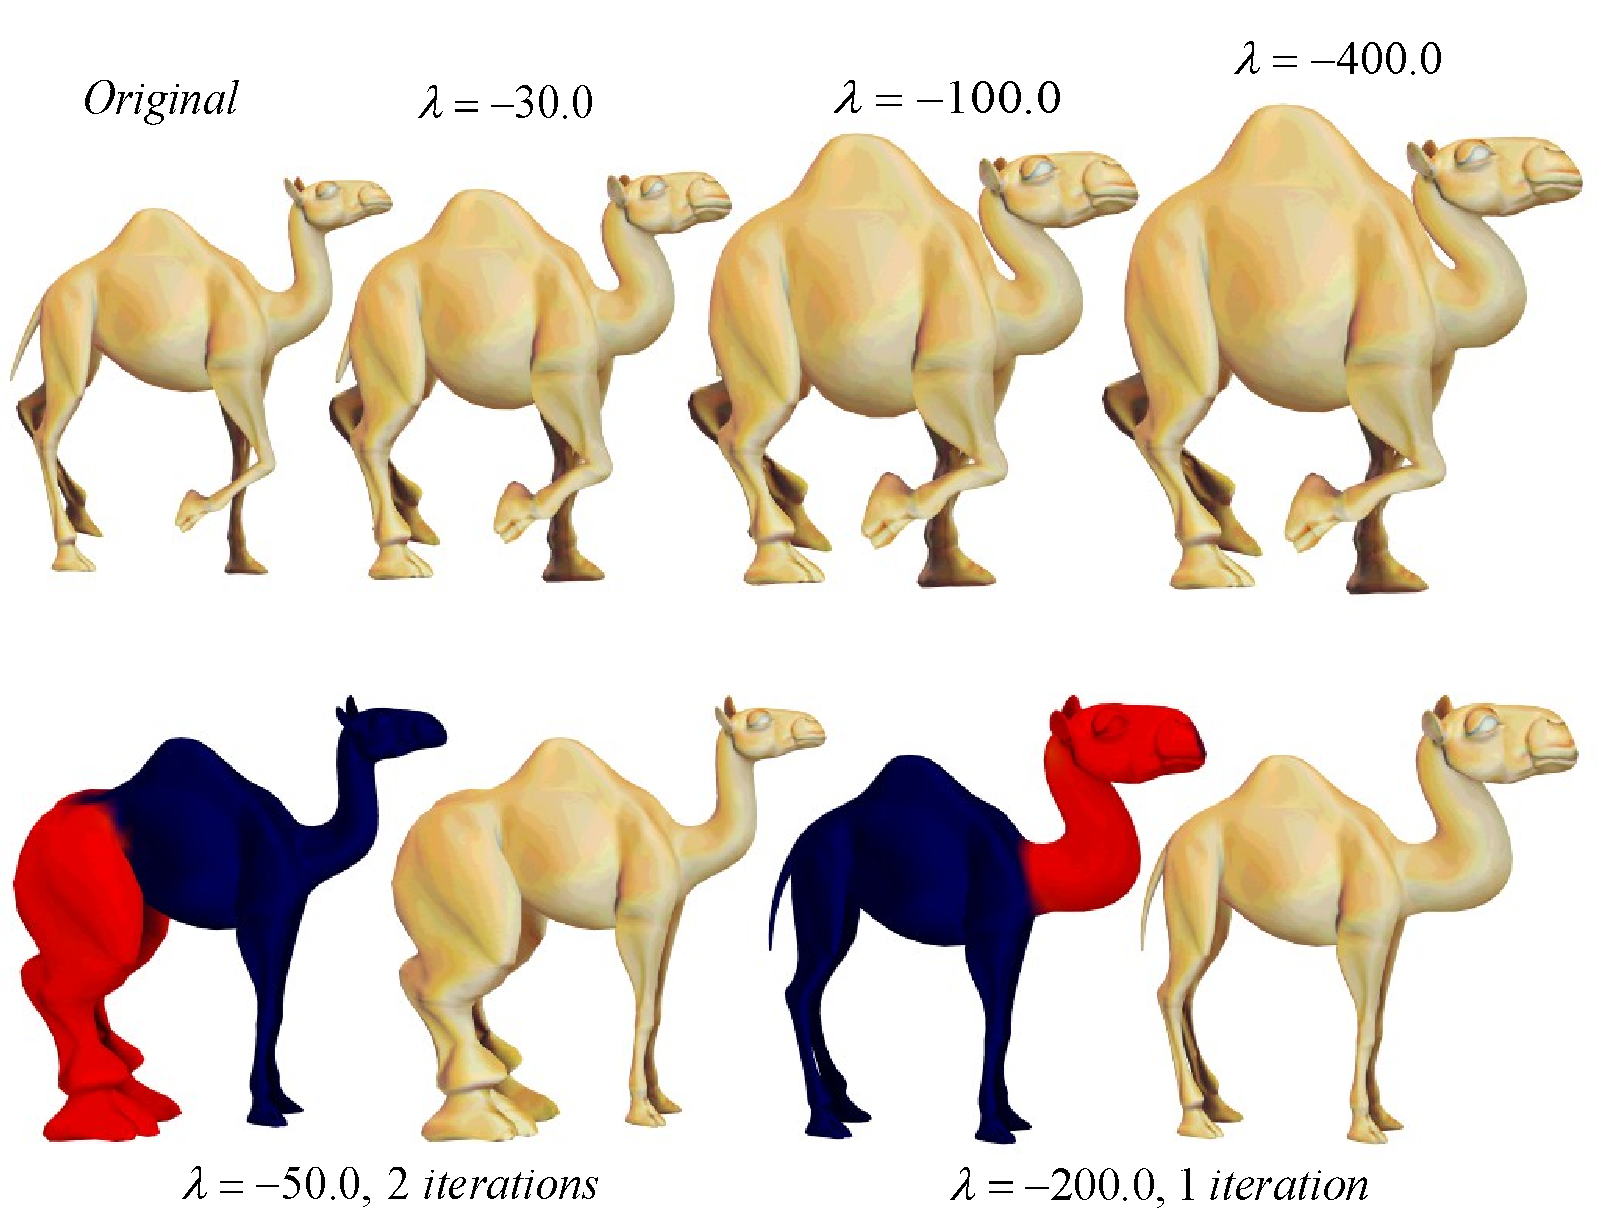
\includegraphics[height=0.5\textheight]{resources/figs/camello_enhanced2}
\par\end{centering}

\caption{\label{fig:camello_enhanced}Top row: Original camel model in left.
Shape inflation with $\lambda=-30.0$, $\lambda=-100.0$, $\lambda=-400.0$.
Bottom row: Shape inflation with weight vertex group, $\lambda=-50.0$
and 2 iterations for the legs, $\lambda=-200.0$ and 1 iteration for
the head and neck.}
\end{figure}


The inflation of the silhouette features is predictable and invariant
under isometric transformations, as those classically used in some
animations (see Figure \ref{fig:Animated_Camell}). In this figure,
the animation shows some camel poses during a walk, the inflation
is performed at the neck and legs, as shown in the bottom left camel
in figure \ref{fig:Animated_Camell}. Local modifications produced
by the pose interpolation or animation rigging practically do not
affect the result. In spite of at any pose of the camel legs there
is a clear difference, the inflation method allows a flesh-like shape
in the original pattern produced by the artist. This is due to the
mesh restricted diffusion process so that small local changes are
treated without affecting the global solution. The method therefore
is rotation invariant since it depends exclusively on the normal mesh
field, which is rotation invariant.

\begin{figure}[H]
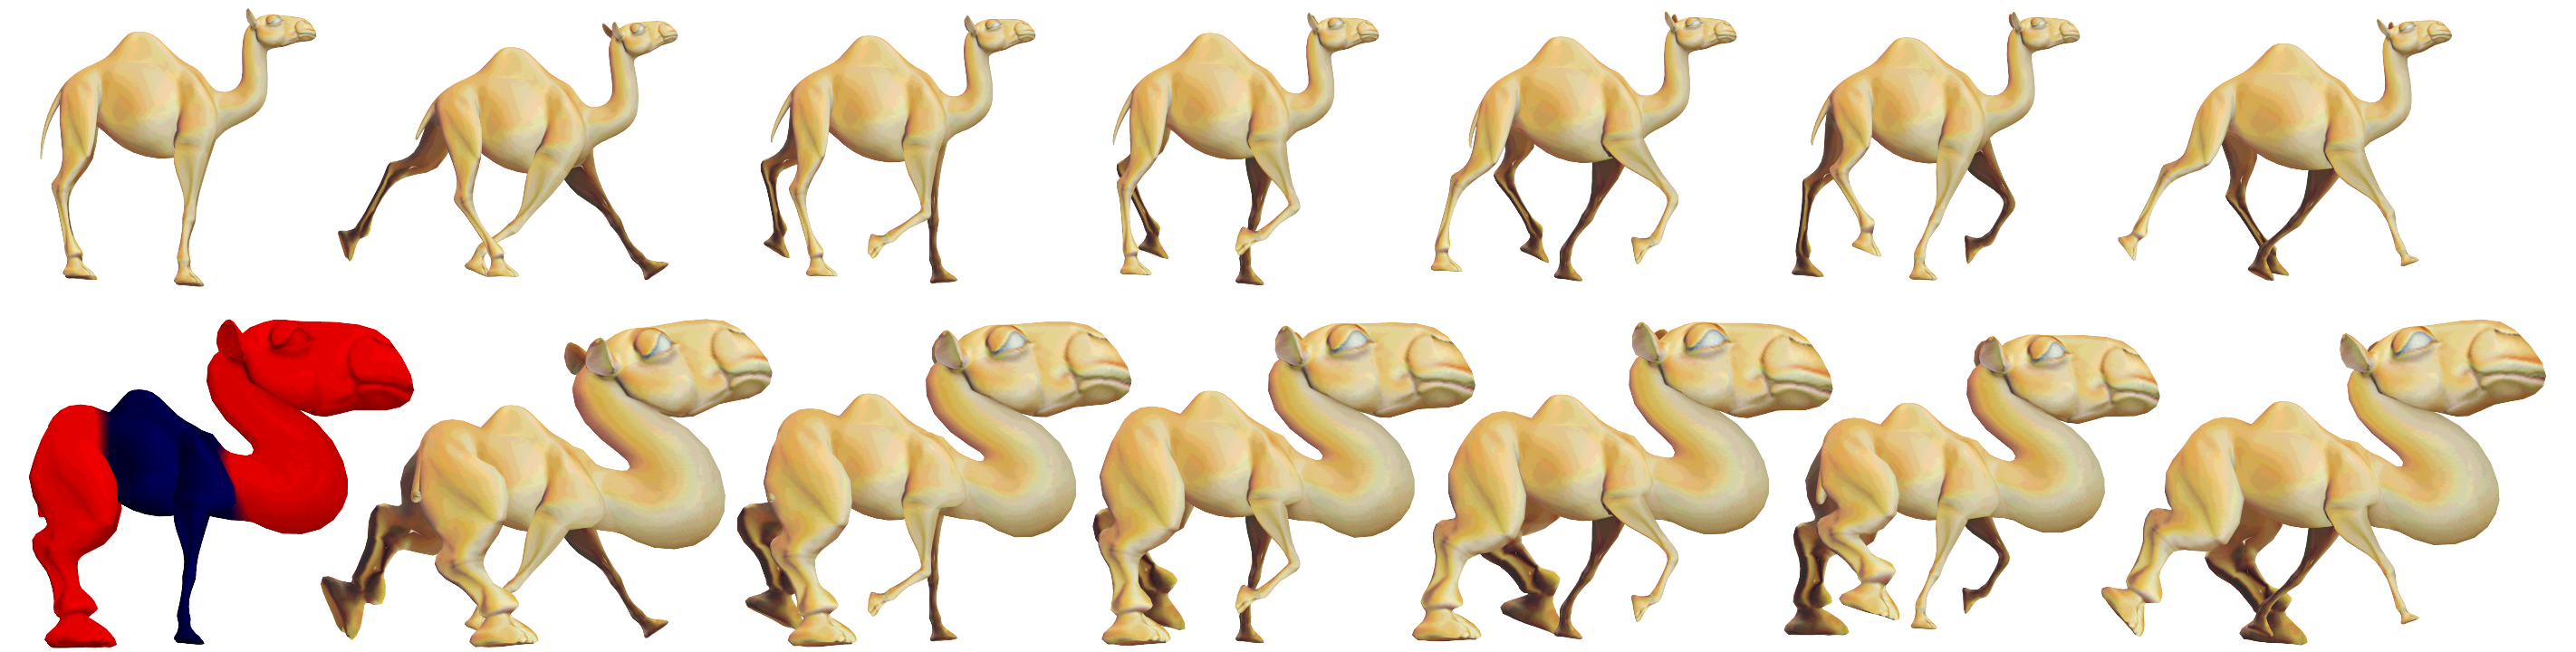
\includegraphics[width=1\textwidth]{resources/figs/camello_walk2}

\caption{\label{fig:Animated_Camell}The method is pose insensitive. The inflation
for the different poses are similar in terms of shape. Top row: Original
walk cycle camel model. Bottom row: Shape inflation with weight vertex
group, $\lambda=-400$ and $2$ iterations. }
\end{figure}



\section{Shape Inflation Brush in Real Time\label{sec:Shape-Inflation-Brush}}

Figure \ref{fig:Sculpt_Brush} shows the use of a shape inflation
brush for sculpting in real time. One pass was used with the brush,
as shown in the figure, with the blue and red radius. In figure \ref{fig:Sculpt_Brush}.b
the camel foot shows the inflation intersection that looks like two
bubbles, a similar pattern to what is observed to the fingers on the
bottom of the same figure. The silhouette inflation is observed in
figure \ref{fig:Sculpt_Brush}.c since the main shape is retained
together with its finger and foot details. Similar results can be
obtained by a user, however it would take several steps and require
the use of several brushes, while the shape inflation took a single
step. Likewise, this new method can easily inflate organic features
like muscles during the sculpting process. In figure \ref{fig:Performance-sculpt}
the shape inflation brush performance is illustrated, in this experiment
three models with 12K, 40K and 164K vertices, were used. These models
were sculpted with the shape inflate brush, at each step the brush
sphere containing a variable number of vertices for processing. The
processing time for 800 vertices in the camel paw (40k model) only
took 0.1 seconds, for 2600 vertices in the leg and neck (model 40k)
took 0.5 seconds, these times are suitable in real applications since
an artist sculpts a model for parts. 

\begin{figure}[H]
\noindent \begin{centering}
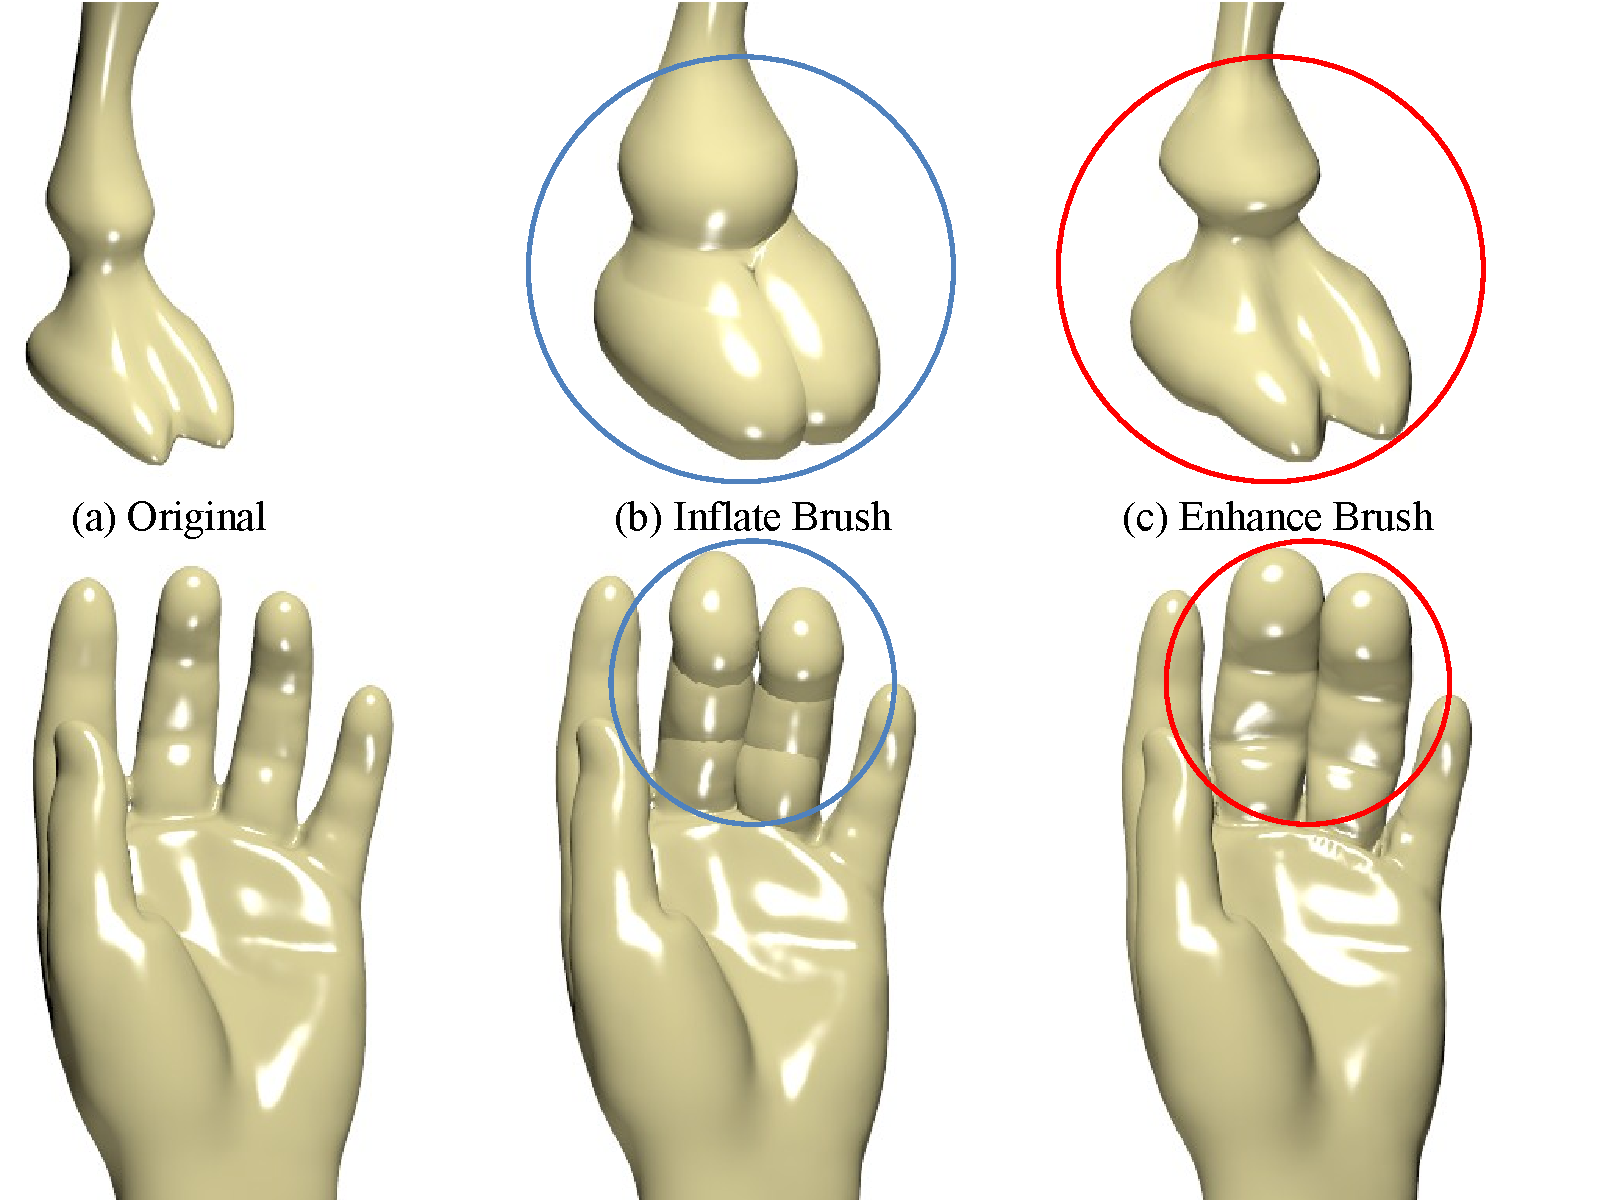
\includegraphics[height=0.3\textheight]{resources/figs/sculpt_brush}
\par\end{centering}

\caption{\label{fig:Sculpt_Brush}Top row: (a) Leg Camel, (b) Inflate brush
for leg into blue circle, (c) Inflate shape brush for leg into red
circle. Bottom row: (a) Hand, (b) Inflate brush for fingers into blue
circle, (c) Shape inflation brush for fingers in red circle.}
\end{figure}


\begin{figure}[H]
\noindent \begin{centering}
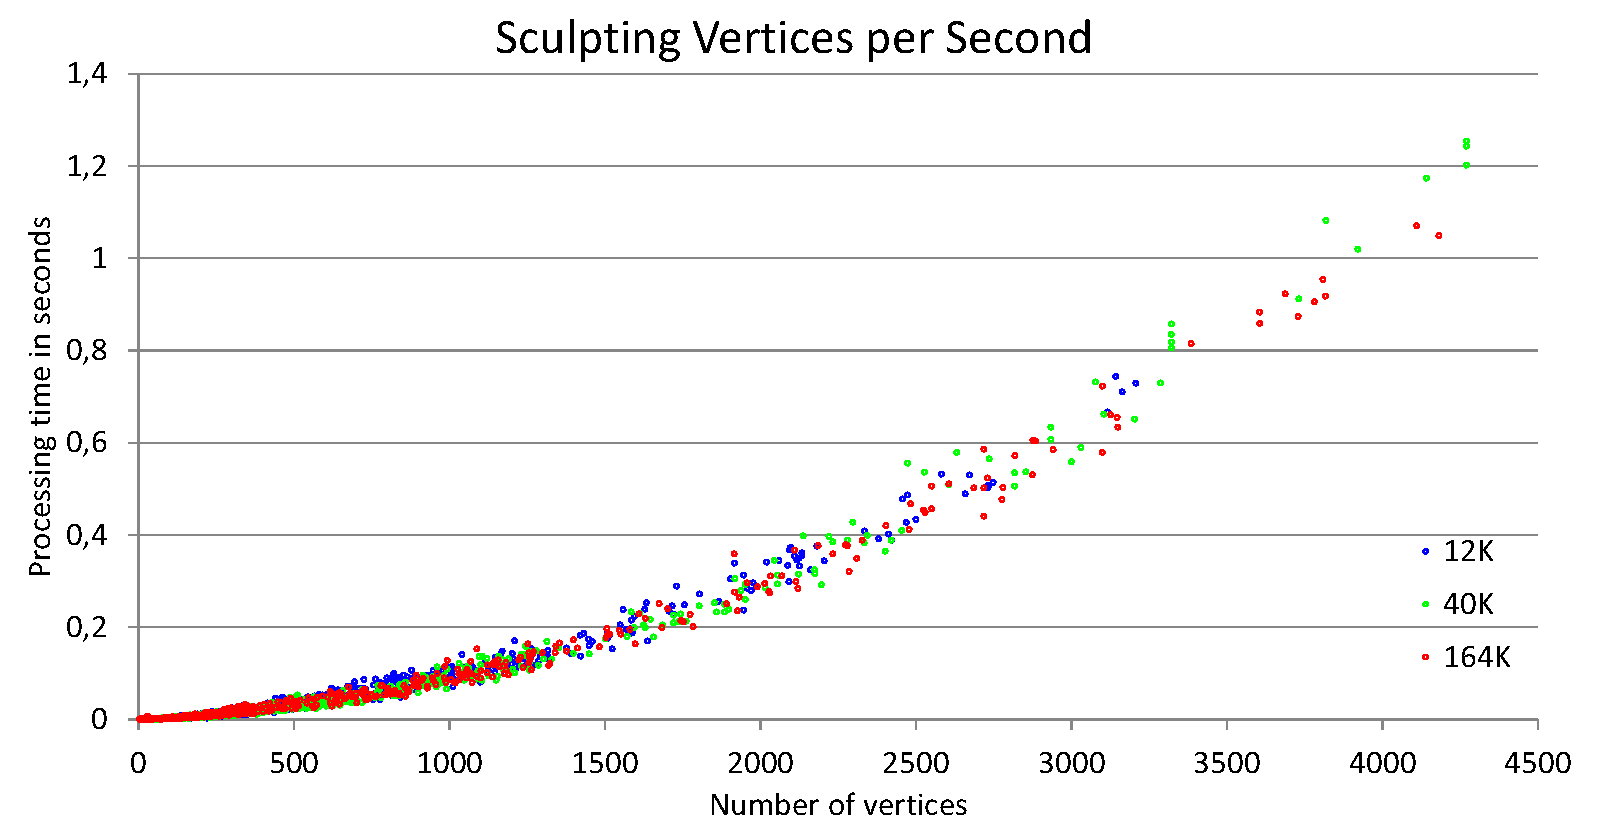
\includegraphics[width=1\columnwidth]{resources/figs/verts_per_second_sculpt}
\par\end{centering}

\caption{\label{fig:Performance-sculpt}Performance of our dynamic shape inflation
brush in terms of the sculpted vertices per second. Three models with
12K, 40K, 164K vertices used for sculpting in real time.}
\end{figure}



\section{Posing Meshes with Laplacian Deform\label{sec:Posing-Meshes-with}}

\begin{figure}[H]
\noindent \begin{centering}
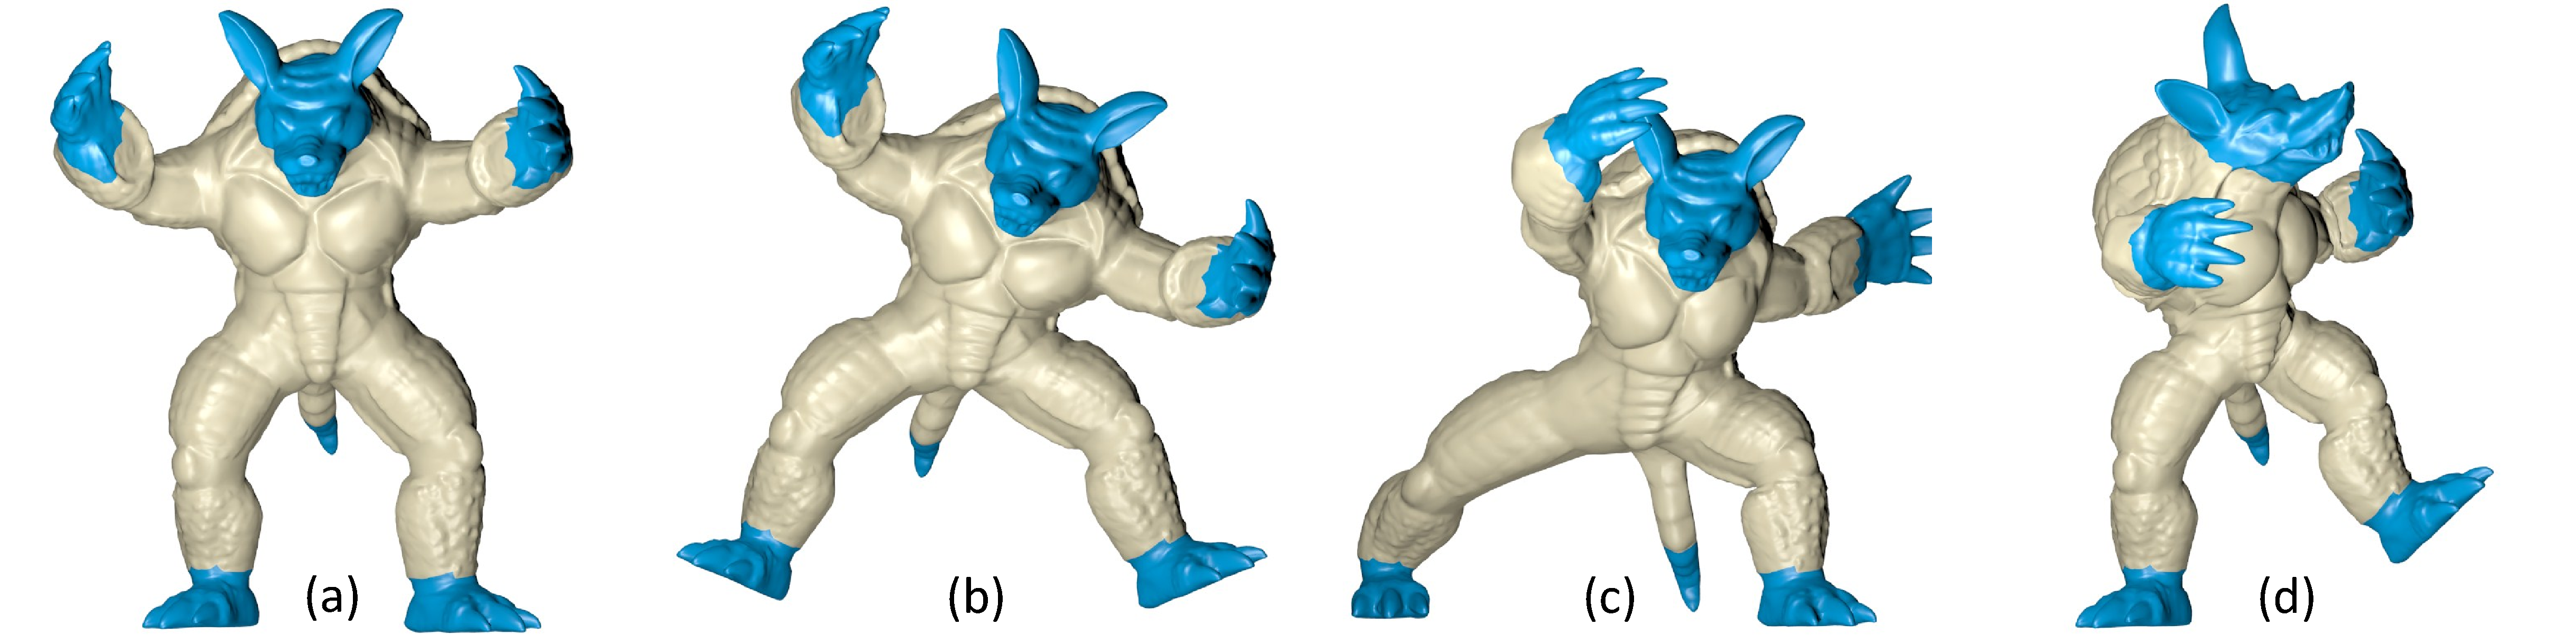
\includegraphics[width=1\textwidth]{resources/figs/Armadillo}
\par\end{centering}

\caption{\label{fig:Armadillo}Anchor vertices in blue color. (a) Original
Model, (b,c,d) new poses change only anchor vertices, system find
positions for vertices in yellow color.}
\end{figure}


Figure \eqref{fig:Armadillo} shows the Laplacian Deform applied in
a model with 173K vertices, only anchor vertices was used and are
represented in blue color, when the user apply several transformation
(location, rotation, scale) over this anchors vertices, the system
find a solution and estimate the position of the vetices in yellow
color. This method work in real time, to achieve this the matrix $\begin{bmatrix}w_{l}L\\
W_{c}
\end{bmatrix}$ in the equation \eqref{eq:LaplacianDefomSystem} is decomposed in
matrix $LU$ with LU factorization only one time when the system init.
Once the matrix is factorized the system can solve the unknowns in
a fast way in term of miliseconds. For get better results the method
permits solve several times the system of equations, and not need
factorize matriz LU could be that at every iteration, only the differential
coordinates are adjust since the differential coordinates can be rotated
at every iteration and get bettter results. In the figure only four
iterations were used, but the system find good solutions with only
one iteration when the angle of rotations are less that $\pi$.


\section{Laplace Operator and Normalized Version \label{sec:Laplace-Operator-and}}

Tests with the Laplacian operator (equation \ref{eq:TQLBO_Simple_Matrix})
and its normalized version (equation \ref{eq:TQLBO-Normalized_Matrix}),
produce similar results if the triangles or quads that compose the
mesh are about the same size. The normalized version is more stable
and predictable because it is not divided by the area of the ring
which may be very small and causes numeric problems, as shown in figure
\ref{fig:(a)Monkey}.c bottom row. The shape inflation of the model
with the normalized Laplacian operator results in a more regular pattern.
The model can be deformed with a TQLBO normalized version with large
$\lambda$ ($\lambda>400$) while intersecting itself with no peaks.
Figure \ref{fig:(a)Monkey}.c shows different results due to the quads
areas in the model. Quadss with larger area have smaller inflation
(figure \ref{fig:(a)Monkey}.c skull), and smaller quads have larger
inflations (figure \ref{fig:(a)Monkey}.c chin).

\begin{figure}[H]
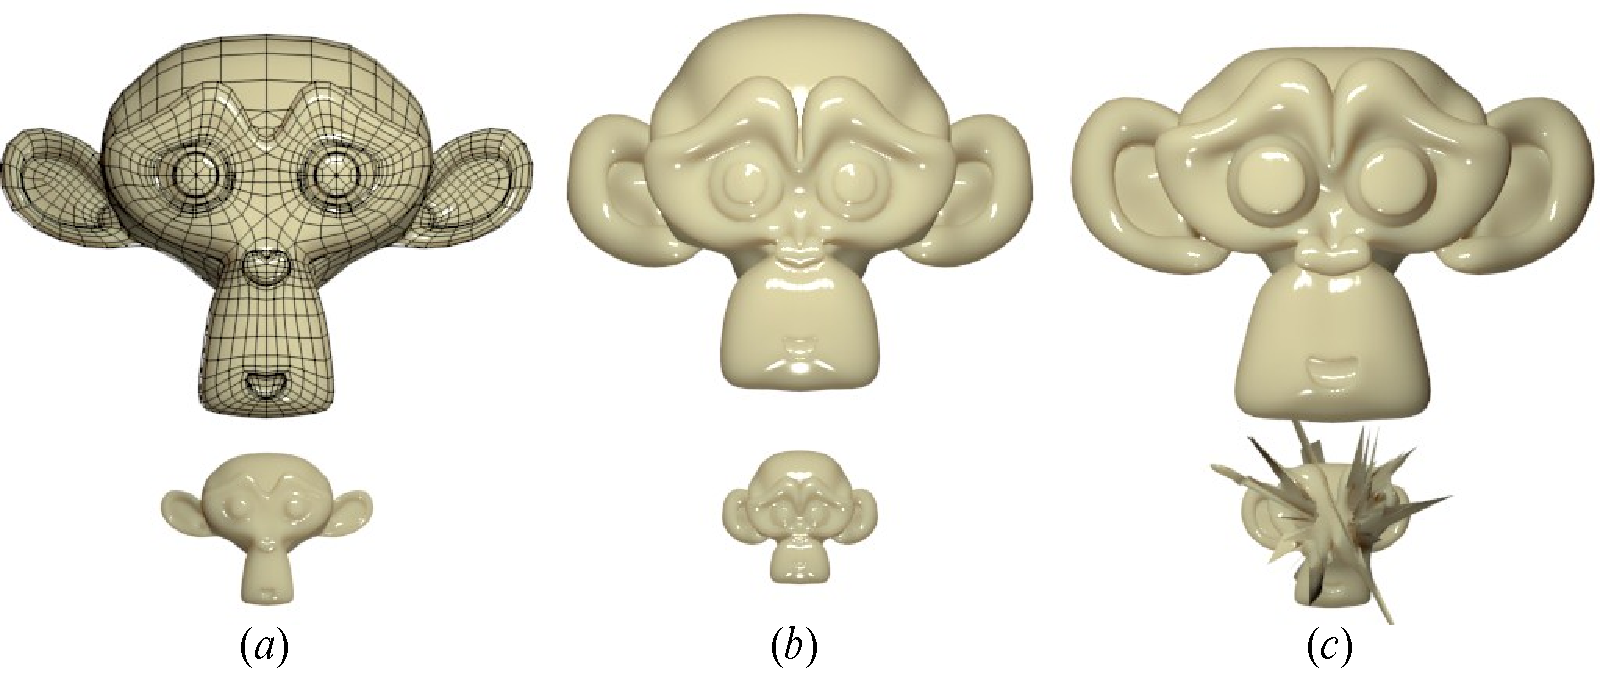
\includegraphics[width=1\columnwidth]{resources/figs/monkey}

\caption{\label{fig:(a)Monkey}(a) Bottom row: Original Model. Top row: Original
model scaled by 4. (b) Top and bottom row: inflating with Normalized-TQLBO
$\lambda=-50$ (c) Top and bottom row: inflating with TQLBO $\lambda=-50$.}
\end{figure}



\section{Skeletonizer}

Skeletonizer is a product of software that permits the proccessing,
visualization and extraction of the skeleton from polygonal meshes.
The software was designed with base in a plugin system and pipe-filters
paradigm. This software implement the method for skeleton extraction
describe in equation \ref{eq:SkeletonExtractionDistance}.

The software is called sjSkeletonizer and use the following computacional
frameworks and libraries.
\begin{description}
\item [{CGAL}] Computational Geometry Algorithms Library \cite{cgal}.
\item [{Graphite}] is a research platform for computer graphics, 3D modeling
and numerical geometry \cite{graphite}.
\item [{QT}] is a cross-platform application and UI framework \cite{qt}.
\end{description}
\begin{figure}
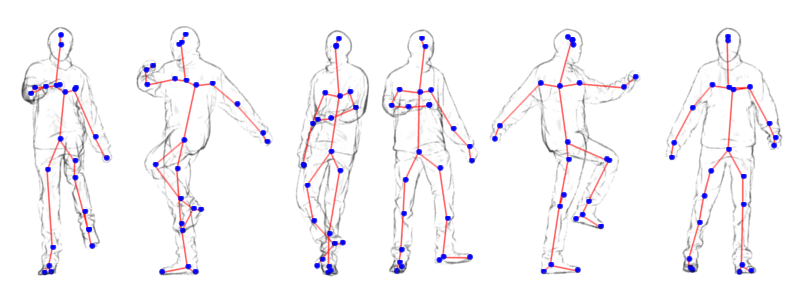
\includegraphics[width=1\textwidth]{resources/figs/poses}

\caption{\label{fig:Skeleton-extraction-poses} Model with different poses
and skeleton obtained with our skeleton extraction software.}


\end{figure}



\section{Performance Testing of Solvers \label{sec:Performance-Testing-of}}

Performance evaluation of some numerical solvers for compute Laplacian
Smooth system.

Linear equation system to solve

$\frac{\partial V}{\partial t}=\lambda L\left(V\right)$

Integrating the diffusion equation with a explicit Euler scheme

$\left(I-\lambda\partial tL\right)V^{n+1}=V^{n}$

Where $V^{n+1}$ is the actual position of vertices, and $V^{t+1}$
are the vertices after Laplacian Smoothing. $\lambda\partial t$ is
the smoothing factor. L is the Laplacian Matrix defined in equation
\ref{eq:TQLBO_Simple_Matrix}.

Solving the sparse linear system

$Ax=b$

Where:

$A=\left(I-\lambda\partial tL\right)$

$x=V^{n+1}$

$b=V^{n}$


\subsection{Hardware Specification }
\begin{itemize}
\item Processor: AMD Quad-Core 2.40 GHz 
\item RAM: 8.0 GB 
\item OS: Windows 7 Professional 
\item Graphics controller: NVIDIA Quadro FX 570
\end{itemize}

\subsection{Software Specification }
\begin{description}
\item [{CGAL}] Computational Geometry Algorithms Library 
\item [{Graphite}] Research platform for computer graphics
\end{description}

\subsection{Numeric Solvers Used }
\begin{description}
\item [{CG:}] Conjugate gradient method. 
\item [{BICGSTAB:}] Biconjugate gradient stabilized method. 
\item [{GMRES:}] Generalized minimal residual method. 
\item [{SUPERLU:}] Sparse Direct Solver, LU decomposition with partial
pivoting. 
\item [{TAUCS\_LDLT:}] A library of sparse linear solvers with LDLT factorization. 
\item [{CHOLMOD:}] Supernodal sparse Cholesky factorization. 
\end{description}
LU factorization is a numerical method that works with large, sparse,
nonsymmetric systems of linear equations \cite{Levy2005}. We choose
the implementacion of LU factorizacion in a OpenNL-SuperLU library,
because this method show the better performance for the computacion
of a solution for a Laplacian Smoothing linear system of equations
presented in equation \ref{eq:LaplacianSmoothLinearEquationSystem}
how see in the table \ref{tab:TimeVsSolvers}. OpenNLSuper allow works
with the Graphics Unit Proccesor GPU, for exploit the capacity of
GPU to work with parallel structures, more fast that traditional CPU.

\begin{table}[H]
\begin{tabular}{|c|c|c|c|c|c|c|c|}
\hline 
Model & Vertices & CG & BICGSTAB & GMRES & SUPERLU & TAUCS & CHOLMOD\tabularnewline
\hline 
\hline 
Cross & 24 & 0.05 & 0.05 & 0.04 & 0.04 & 0.05 & 0.05\tabularnewline
\hline 
King & 538 & 0.83 & 0.63 & 0.71 & 0.61 & 0.68 & 0.79\tabularnewline
\hline 
YModel & 4770 & 19.60 & 16.44 & 16.93 & 16.06 & 16.88 & 17.95\tabularnewline
\hline 
Man & 10002 & 33.43 & 27.76 & 29.91 & 28.54 & 29.53 & 30.80\tabularnewline
\hline 
Neptune & 28052 & 133.97 & 136.46 & 136.39 & 133.21 & 142.87 & 142.76\tabularnewline
\hline 
Armadillo & 34594 & 194.48 & 174.88 & 175.80 & 169.92 & 181.70 & 183.49\tabularnewline
\hline 
\end{tabular}

\caption{\label{tab:TimeVsSolvers}Vertices Vs Seconds, Laplacian Smoothing
performance.}
\end{table}


\begin{figure}[H]
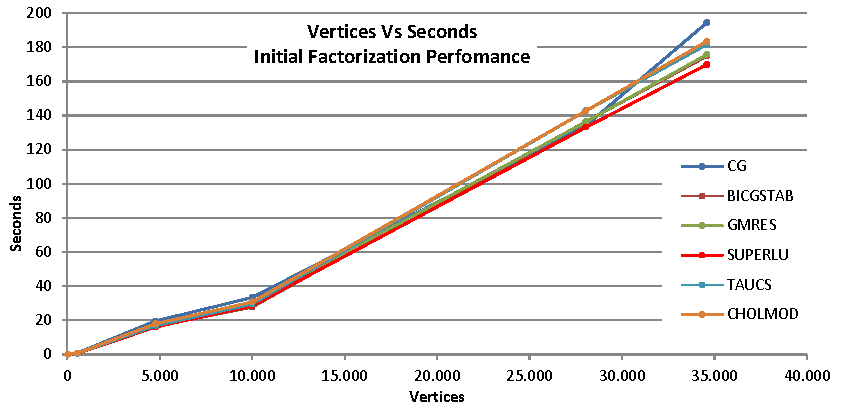
\includegraphics[width=1\textwidth]{Data/Benchmark}

\caption{asdas}


\end{figure}



\section{Implementation\label{sec:Implementation}}

The method was implemented as a modifier for modeling and brush for
sculpting, on the Blender software \cite{blender} in C and C++. Working
with the Blender allowed to test the method interactively against
others, as Catmull-Clark, weight vertex groups and sculpting system
in Blender.

To improve the performance, it was worked with the Blender mesh struct,
visiting each triangle or quad and storing its corresponding index
and the sum of the Laplacian weights of the ring in a list so that
only two visits were required for the list of mesh faces and two times
the edge list, if the mesh was not closed. This drastically reduced
calculations, enabling real-time processing. In the construction of
the Laplacian matrix, several index were locked at vertices having
face areas or edge lengths with zero value that could cause spikes
and bad results.

Under these conditions, the matrix at equation \ref{eq:TQLBO_Simple_Matrix}
is sparse since the number of neighbors per vertex, corresponding
to the number of data per row, is smaller compared to the total number
of vertices in the mesh. To solve the linear system equation \ref{eq:Lineal_System_with_wp}
was used OpenNL which is a a library for solving sparse linear system.


\chapter{Conclusion and future work\label{sec:Conclusion-and-future}}

This work presented an extension of the Laplace Beltrami operator
for hybrid quad/triangle meshes that can be used in production environments
and provides results similar to those obtained by working only with
triangles or quads. This paper has introduced a new way to change
silhouettes in a mesh for modeling or sculpting in a few steps by
means of the curvature model modification while preserving its overall
shape. In addition, a new modeling method has also been presented
some possible applications have been illustrated. The method works
properly with isometric transformations, opening the possibility of
introducing it on the process of animation.

We show that this tool may work in early modeling stages, case in
which coarse models are used, allowing to modify the shape generated
by the Catmull-Clark subdivision surfaces, and thereby avoiding edition
of the vertices with change of a single parameters.

Future work includes the analysis of theoretical relationships between
the Catmull-Clark subdivision surfaces and the Laplacian smoothing
since they can produce very similar results. 

\bibliographystyle{plain}
\addcontentsline{toc}{chapter}{\bibname}\bibliography{bibliografia/listado_inicial,TQLBO-paper/template,D:/src/blender/GSoC/GSOC2013/bibliography_mesh_editing,SIBGRAPI2013/template}

\end{document}
